% ============================================================
%  基于人工智能的黑土地遥感动态变化监测系统 —— 项目计划书
%  编译方式：xelatex 项目计划书.tex（建议连续编译两次以生成目录）
%
%  本文件为【带图版】：正文中原图片位置已替换为真实图片引用，
%  图片位于 ./项目计划书图片/ 目录，可直接 xelatex 编译出带图成品。
%  （保留图片空位的版本见 项目计划书.tex）
% ============================================================
\documentclass[12pt, a4paper]{ctexart}

\usepackage[top=2.5cm, bottom=2.5cm, left=2.8cm, right=2.8cm, headheight=15pt]{geometry}
\usepackage{graphicx}
\usepackage{float}
\usepackage{array}
\usepackage{booktabs}
\usepackage{enumitem}
\usepackage{caption}
\usepackage{fancyhdr}
\usepackage{eso-pic}
\usepackage{pdfpages}
\usepackage[hidelinks]{hyperref}

\captionsetup{font=small, labelsep=quad}
\setcounter{secnumdepth}{-1}   % 章节目录编号由正文手写（一、二、…），关闭 LaTeX 自动编号
\pagestyle{fancy}
\fancyhf{}
\fancyhead[C]{\small 黑土地遥感动态变化监测系统 · 项目计划书}
\fancyfoot[C]{\thepage}
\renewcommand{\headrulewidth}{0.4pt}

\title{\vspace{-1.2cm}
  {\large\heiti 中国国际大学生创新大赛（2026）}\\[0.5em]
  {\normalsize 赛道：国家级产业赛道　组别：成果转化组}\\[1.4em]
  {\heiti 基于人工智能的黑土地遥感动态变化监测系统}\\[0.4em]
  {\large\heiti 项目计划书（创意策划方案）}}
\author{汤福连 \quad 刘芮仲 \quad 于欣欣 \quad 张珏枫}
\date{\today}

\begin{document}

% ===== 封面（整页一张）：设计稿 + 大赛信息 + 团队成员，与扉页合并为一页 =====
% fitpaper 使该页尺寸与封面 PDF 完全一致；更换封面后请重新运行 .claude/make_cover.py
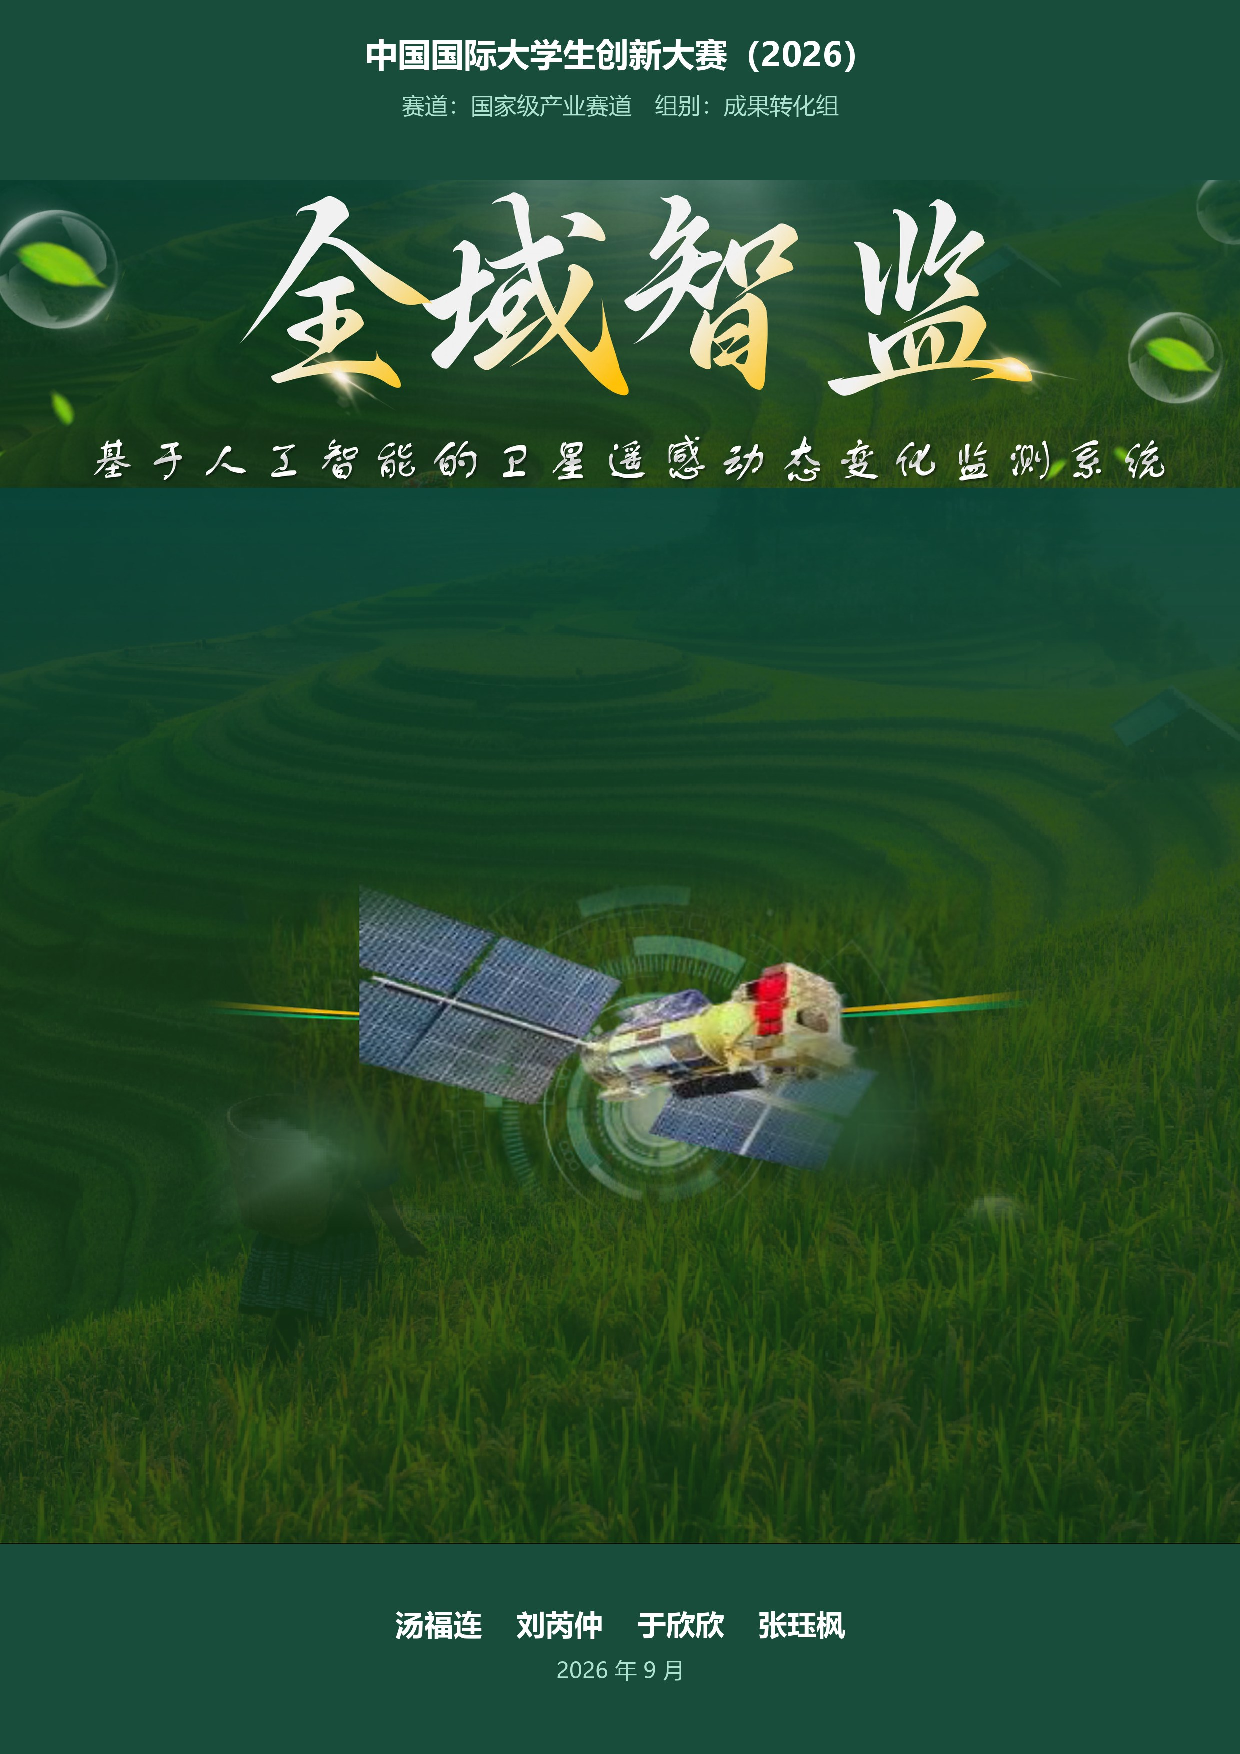
\includepdf[pages=1, fitpaper=true]{项目计划书图片/封面.pdf}

% ===== 自封面之后的所有页面统一铺淡色背景 =====
% 换浓度只需改文件名：背景淡07.png（最淡）/ 背景淡12.png / 背景淡18.png（纹理最明显）
\AddToShipoutPictureBG{%
  
\includegraphics[width=\paperwidth,height=\paperheight]{项目计划书图片/背景淡12.png}%
}

\tableofcontents
\newpage

% ==================== 片段 g1 ====================
\section{一、摘要}

黑土地是保障国家粮食安全的重要战略资源，东北黑土地作为我国最重要的商品粮基地之一，其土层厚度、有机质含量与结构稳定性的变化，直接关系到区域农业生产的可持续性和国家粮食供给的长期稳定。近年来，随着《中华人民共和国黑土地保护法》的颁布实施，以及《国家黑土地保护工程实施方案（2021—2025年）》《东北黑土地保护性耕作行动计划（2020—2025年）》等系列政策的持续推进，黑土地保护已由局部试点上升为制度化、常态化的国家任务，对监测手段的时效性、覆盖范围与数据可信度提出了更高要求。然而，传统黑土地监测长期依赖人工实地巡查与目视解译，存在人工巡查效率低、光学遥感解译精度不足、数据与治理脱节等核心痛点：人工巡查受人力和交通条件制约，难以覆盖广袤耕地，且判读结果主观性强、复现性差；遥感数据获取能力虽不断增强，却缺乏与之匹配的自动化智能解译手段，致使海量影像“存而不用”，监测结论难以快速转化为可执行的治理决策。监测能力与治理需求之间的这一落差，正是本项目立项所要解决的关键问题。

从量化背景看，黑土地退化的累积效应已经显现：黑土层平均减薄6.83cm（累计值），有机质下降的样点占比达52.5\%，存在水土流失的样点占比达24.4\%。三组数据分别从土层厚度、肥力水平与表土流失三个维度刻画了退化的程度与普遍性，说明黑土地质量下降并非个别地块的偶发现象，而是区域尺度上的系统性问题。退化过程还具有渐变性与分散性：单次实地巡查难以察觉细微差异，而持续累积则可能演变为难以逆转的沟蚀与肥力衰退。因此治理必须建立在“早发现、早干预”的基础上，也要求监测具备周级频次与地块级分辨率，使保护措施能在退化尚处可逆阶段时及时介入。

针对上述痛点，本项目设计了一套基于人工智能的卫星遥感动态变化监测系统，构建“天空地一体化光学遥感采集+AI智能解译+可视化决策支撑”的完整技术闭环。其中，“天空地一体化采集”负责多平台、多时相影像的稳定获取；“AI智能解译”负责将原始影像转化为可量化的变化信息；“可视化决策支撑”负责把变化信息组织为面向基层管理者的直观图件与分析结论。三者相互衔接、逐级递进，形成从数据输入到决策输出的贯通链路。

在技术实现上，系统以国产GF-2亚米级光学遥感卫星影像与无人机航拍影像为核心数据源，以改进BIT双时相Transformer模型为算法核心，搭配ResNet18骨干网络实现高分辨率影像的多尺度特征提取；同时开发了前后端分离的轻量化可视化系统，支持批量影像处理、变化检测、结果可视化与一键生成分析报告，普通计算机即可完成本地化部署，降低了在基层单位推广使用的硬件门槛。经试点验证，系统对黑土地变化识别精确率达70\%，算力成本降低69\%，监测周期缩短33\%，已在黑龙江松嫩平原完成落地应用，可为黑土地常态化保护与精细化治理提供高效、自主可控的光电监测技术支撑，助力保障国家粮食安全。

\section{二、项目概况与核心组成}

\subsection{1.项目总体目标}

本项目面向黑土地保护“精准治理”的现实需求，以“天空地一体化监测+AI智能解译”为核心，开发一套土地光学遥感变化检测智能系统，实现黑土地退化的自动化识别、可视化分析与辅助决策，构建“数据采集—智能检测—分析决策”的完整技术闭环，为黑土地保护提供高效、精准的科技支撑。

上述目标可进一步分解为三个相互支撑的层面。第一是数据采集层面，打通卫星与无人机两类平台的影像获取通道，保证监测区域在时间维度上“有数据可用、有数据可比”；第二是智能检测层面，用深度学习模型替代重复性的人工目视解译，把侵蚀沟发育、植被覆盖变化、土地利用变化等退化信息从影像中自动提取出来，并使检测结果在精度与稳定性上满足业务要求；第三是分析决策层面，将模型输出转化为管理者可直接理解的图件、指标与报告，使监测结论能够进入日常巡查、执法核查与保护性耕作评估等具体工作流程。

需要说明的是，本项目并非面向通用场景的遥感监测平台，而是紧扣黑土地保护业务的专用系统，其差异化定位体现在三个层面。算法层面，通用变化检测模型多以城市扩张、地表覆盖转换等目标优化，本项目则针对侵蚀沟发育、植被覆盖变化、土地利用变化等黑土地退化信息专项训练，使模型关注的类别与业务关注的对象一致。数据层面，通用方案多单依赖卫星影像，受重访周期与云层遮挡制约，本项目以国产GF-2亚米级影像承担周期性普查、以无人机影像承担重点核查。结果层面，通用方案输出多为栅格差异图或矢量图斑，仍需二次判读，本项目则直接输出图件、指标与文字结论，把专业解译封装在系统内部。三方面取舍共同指向同一目标：使不具备遥感背景的基层使用者同样能获得可用的监测结论。

项目目标的设定强调“可用”与“可推广”并重。一方面，系统功能围绕真实业务环节组织，避免停留在算法演示层面；另一方面，系统在算力占用、部署方式与操作复杂度上做了针对性约束，使其能够在算力条件有限的基层单位稳定运行，从而具备从单点试点走向区域推广的现实基础。项目按照既定时间线推进：2022年启动政策调研与数据积累，2024年完成影像标注与模型验证，2026年获软件著作权并落地试点，2028年推广至黑吉辽蒙四省区，2030年构建“天空地”一体化监测网。

从成果基础看，项目并非从零起步。团队围绕遥感变化检测与监测系统开发已形成自主知识产权积累，累计获得软件著作权3项，并取得实用新型专利1项（专利号ZL 2025 2 2047856.0，授权公告号CN 224511490 U，专利权人为黑龙江八一农垦大学）。相关权利覆盖算法实现、系统软件与装置结构等层面，表明项目在原理验证与工程实现上均已具备可核验的基础，为后续推广提供了支撑。

\subsection{2.项目核心组成部分}

围绕上述目标，项目由AI算法核心、多源数据支撑、可视化智能系统三部分组成。三者分别对应“算得准”“看得清”“用得上”三个环节，共同构成完整的技术链条。

三者之间并非简单的功能并列，而是相互约束、彼此支撑的有机整体。算法对数据提出要求：Transformer模型需要在有限算力下完成全局建模，就要求影像在空间分辨率与时间一致性上达到一定标准，这直接决定了采集环节对GF-2亚米级影像与无人机核查影像的取舍；数据反过来检验算法：多时相、多平台的影像覆盖，使模型可能遇到的成像差异与季节变化被充分暴露，从而推动训练策略的持续调整。算法与数据共同支撑系统：只有模型输出稳定、数据基础可靠，可视化系统呈现的图件与结论才具备决策价值；而系统的实际使用又会反馈新的疑点与误差样本，为模型迭代提供标注来源。三者由此形成“数据喂养算法、算法支撑系统、系统反馈数据”的闭环，任何一环的削弱都会影响最终治理决策的可靠性。

\subsubsection{（1）AI算法核心：基于Transformer的深度学习模型}

以BIT（Bipartite Transformer）深度学习模型为算法核心，针对黑土地遥感影像的特征进行优化训练，实现对侵蚀沟、植被覆盖变化、土地利用变化等关键退化信息的高精度、自动化检测，解决传统人工解译效率低、主观性强的问题。

从技术原理看，变化检测的本质是对同一区域两个不同时相的影像进行逐像素的对应分析与差异判别。卷积神经网络虽擅长提取局部纹理与边缘特征，但其感受野受限于卷积核尺寸，对影像中大范围、长距离的空间关联刻画不足，容易在连片的耕地与沟道区域出现漏检或边界模糊。BIT双时相Transformer模型\cite{ref1}通过自注意力机制建模任意两个位置之间的依赖关系，能够在整幅影像范围内建立全局上下文联系，从而更准确地判断“变化区域是什么、变化边界在哪里”。模型中引入的语义分词器（semantic tokens）负责将影像特征归纳为一组高层语义表示，以此约束注意力计算的范围并保留类别语义信息；ResNet18骨干网络则负责从高分辨率影像中提取多尺度特征，兼顾细节纹理与宏观结构。二者的组合在保持Transformer全局建模能力的同时，抑制了计算量的膨胀，为在有限算力条件下完成推理提供了可行路径。

在训练环节，模型针对黑土地遥感影像的成像特点与地物分布规律进行专项优化：考虑不同季节植被覆盖差异、地表含水量变化以及云雾干扰等因素对影像色调的影响，通过标注样本的扩充与训练策略的调整，提升模型在复杂成像条件下的稳定性与泛化能力。与人工目视解译相比，模型不受主观经验差异影响，判读标准统一、结果可复现，且可批量处理连续时相影像，为周级动态监测提供了算法基础。

在方案取舍上，项目选择CNN骨干与Transformer注意力相结合，而非纯卷积或纯注意力的单一路线，原因在于黑土地遥感影像同时包含两类信息：地块边界、沟道边缘等依赖局部细节的纹理特征，以及连片耕地、沟系走向等依赖大范围空间关联的结构特征。纯卷积结构对后者刻画不足，纯注意力结构则在高分辨率影像上算力开销过大。以ResNet18骨干提取多尺度局部特征、由语义分词器汇聚高层语义、再交由双时相注意力完成差异判别，使模型在精度与算力之间取得平衡，这也是系统能够在普通计算机上完成推理、进而支撑本地化部署的前提。

\subsubsection{（2）多源数据支撑：“天空地”一体化光学遥感采集}

以高分辨率光学遥感影像为核心数据源，构建多平台协同采集体系：

\begin{itemize}
    \item 卫星端：支持GF-2等国产高分辨率卫星的批量数据处理，实现大范围周期性的黑土区动态监测；
    \item 无人机端：完成算法的机载适配，支持野外现场快速检测，弥补卫星数据重访周期长、受天气影响大的短板，实现重点区域的精细化核查。
\end{itemize}

两类平台在观测尺度与响应速度上形成互补。卫星平台观测范围大、成像稳定，适合承担区域性的周期性普查任务，其亚米级分辨率足以支撑耕地地块尺度上的变化识别；无人机平台部署灵活、受云层遮挡影响小，可在卫星影像存疑或天气条件不佳时快速抵达现场，对疑似变化图斑进行低空高分辨率复核。由此形成“卫星普查发现疑点、无人机核查确认结果”的作业模式，既保证了监测覆盖面，又提高了结论的确定性。同时，两类数据统一纳入同一套预处理与解译流程，避免因数据来源不同而产生的标准不一致问题，为后续算法处理与结果比对奠定一致的数据基础。

\subsubsection{（3）可视化智能系统：全流程闭环应用开发}

\begin{figure}[htbp]
    \centering
    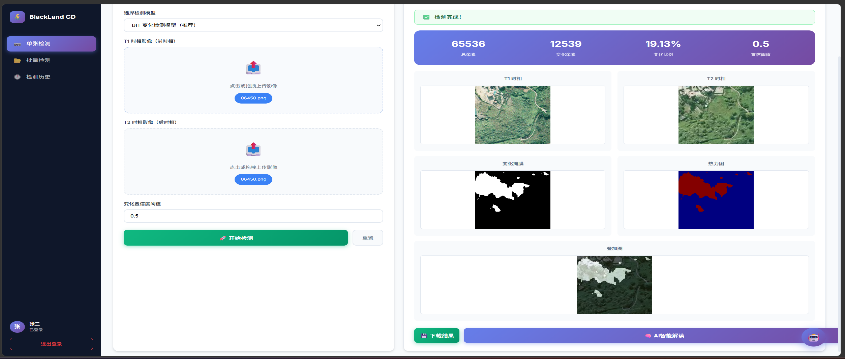
\includegraphics[width=0.8\textwidth]{项目计划书图片/image1.png}
    \caption{黑土地智能监测系统核心功能界面展示}
    \label{fig:1}
\end{figure}

开发并测试了一套可视化智能系统，集成了从数据处理到结果输出的全流程功能：

\begin{itemize}
    \item 支持单张/批量遥感影像变化检测；
    \item 提供结果可视化展示、AI智能解译与一键生成分析报告的功能；
    \item 实现从数据输入到决策支撑的自动化流程，降低用户使用门槛，提升监测效率。
\end{itemize}

系统采用前后端分离的轻量化架构：后端基于FastAPI构建，负责影像接收、任务调度、模型推理与结果组织，接口结构清晰、便于维护与扩展；前端为可视化Web系统，围绕“影像上传—变化检测—结果可视化—AI解读—一键报告”组织操作流程，用户无需掌握遥感专业知识即可完成一次完整的监测作业。批量检测功能解决了连续时相、多个图斑的重复操作问题，使模型的批量推理能力能够真正转化为业务效率；AI解读环节把模型输出的变化图斑转述为自然语言结论，帮助基层人员理解变化的位置、类型与可能成因；一键报告则将影像、图斑与结论自动汇总为规范文档，便于上报归档与横向比对。上述设计使系统从单一的算法工具转变为面向决策的完整应用，普通电脑即可本地化部署，为黑土地保护的常态化监测与精细化治理提供了可持续运转的技术支撑。

% ==================== 片段 g2 ====================
\section{三、项目调研与需求分析}

项目立项之初，团队即确立了“先摸清底数、再定义产品”的工作原则，围绕“现状数据调研”与“多方需求调研”两条主线同步开展工作：前者回答“问题有多严重、为什么必须用新的手段解决”，后者回答“系统应该做成什么样、由谁来用”。两条主线的结论彼此印证，共同构成了本项目技术路线与功能设计的现实依据。

\subsection{1.现状数据调研：黑土地退化问题的量化验证}

为精准把握黑土地保护的现实痛点，项目针对黑龙江黑土区开展了专项调研。该区域地处松嫩平原，是我国东北黑土带的核心分布区之一，也是本项目后续试点落地的目标区域，其退化状况具有典型性与代表性。调研以遥感影像解译与地面观测资料相结合的方式展开，将原本依赖定性描述的退化趋势转化为可度量、可比较的量化指标，数据结果如下图所示。

在调研方法上，团队采用“遥感解译为主、地面资料为辅”的复合方式：一方面选取覆盖松嫩平原典型黑土区的多期国产高分二号（GF-2）亚米级光学遥感影像，通过多时相对比提取地表覆盖变化信息，识别土层裸露、侵蚀沟发育与植被覆盖度下降等退化迹象；另一方面收集整理区域内长期积累的地面观测记录与土壤普查资料，对遥感判读结果进行抽样校核，降低单一数据源可能带来的误判风险。在样本构成上，调研兼顾了地形地貌与耕作方式的差异，既包含地势平坦、连片耕作的代表性地块，也覆盖坡耕地与侵蚀沟发育相对集中的敏感区域，使结论既能反映区域整体趋势，也能揭示退化在空间分布上的不均匀性。以下三项指标，即为上述方法下形成的核心研判结论。

\begin{figure}[htbp]
    \centering
    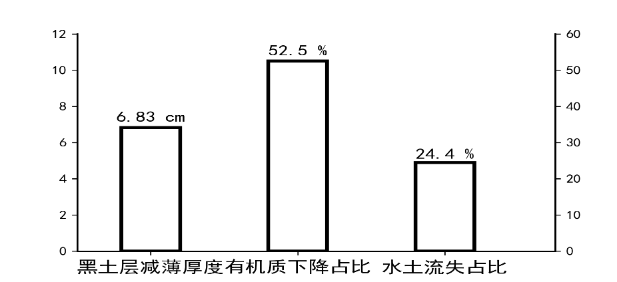
\includegraphics[width=0.8\textwidth]{项目计划书图片/image2.png}
    \caption{黑龙江黑土区退化状况专项调研统计数据}
    \label{fig:img2}
\end{figure}

调研结果显示，黑龙江黑土区退化形势严峻，主要体现在以下三个方面：

\begin{itemize}
    \item \textbf{土层变薄}：黑土层平均减薄厚度达6.83cm，远超自然侵蚀速度。黑土层的形成需要长期腐殖质积累，而流失却可能在数个耕作季内发生，这一减薄幅度直接压缩了作物根系的发育空间与养分供给基础。
    \item \textbf{肥力下降}：土壤有机质含量下降占比达52.5\%，近半数耕地出现明显肥力衰退。有机质降低会同步削弱土壤的保水保肥能力与团粒结构稳定性，往往表现为化肥施用量被动增加而产量提升有限。
    \item \textbf{水土流失}：水土流失问题突出，占比达24.4\%，侵蚀沟扩张对耕地造成直接破坏。侵蚀沟不仅切割地块、阻断农机作业通路，还会将富含有机质的表土持续搬运出境，形成“越冲越薄、越薄越冲”的恶性循环。
\end{itemize}

从成因上看，三项退化指标并非彼此孤立，而是相互耦合、互为因果。长期高强度翻耕使耕层土壤结构被反复扰动，有机质矿化速度加快、团聚体稳定性下降，土壤一旦遭遇降雨便更易被径流带走，这既解释了有机质下降与水土流失在空间上的高度重叠，也说明土层减薄并非单纯的自然过程，而是耕作方式、种植结构与自然侵蚀共同作用的结果。从治理含义上看，这一耦合关系决定了黑土地保护不能停留在单点补救：若只关注肥力指标而忽视侵蚀沟的扩展，施入的有机物料仍会随表土流失而难以积累；若只治理侵蚀沟而不改变耕作方式，新的侵蚀仍会持续发生。因此，治理必须以地块为单元、以时间序列为线索，持续跟踪土层厚度、有机质含量与侵蚀状况的动态变化，才能判断措施是否真正见效并及时调整。这对监测能力提出了新的要求——不仅要“看得清”，还要“看得勤、看得准、看得出趋势”，从而把治理从经验驱动逐步转向数据驱动。

这些量化数据，直观印证了黑土地“变薄、变瘦、变硬”的严峻趋势。需要指出的是，退化问题的紧迫性不仅来自数据本身，更来自监测能力的滞后：传统黑土地监测主要依靠人工实地巡查与逐级上报，存在采样点稀疏、更新周期长、空间覆盖不连续、人力与时间成本高等固有短板，难以在退化发生的早期阶段发现苗头，也无法支撑以地块为单元的精细化治理决策。正是这一“问题在加速、手段在滞后”的错位，为本项目的研发提供了明确的现实依据，也决定了项目必须走“高分辨率遥感 + AI 智能解译 + 快速更新”的技术路线。

\subsection{2.多方需求调研：明确项目落地的实际场景}

为确保项目成果可落地、可推广，项目同步开展了多渠道需求调研，将农户、基层农技人员、土地管理部门以及农业科技企业等不同主体纳入调研范围，力求从“使用者”和“服务者”两个视角交叉验证需求，避免技术方案与真实场景脱节。

两类调研在问题设定上各有侧重：问卷调查面向数量众多的一线使用者，回答的是“需求有多普遍、痛点集中在何处”的问题，其价值在于样本覆盖面广、反馈口径统一，能够从大量分散的意见中提炼出共性诉求；企业走访面向技术供给方与治理实施方，回答的是“现有方案为什么不够用、落地时会受哪些约束”的问题，其价值在于能够接触真实项目中的部署环境、运维条件与成本结构，从而避免方案设计停留在理想条件。前者告诉团队“该做什么”，后者告诉团队“能做成什么”，两条线索相互约束，才共同划定了既先进又可行的设计边界。

\begin{enumerate}
    \item \textbf{问卷调查}：面向农户、基层农技人员、土地管理部门发放问卷，了解一线监测的痛点。调研反馈集中指向三类问题：一是人工巡查效率低，地块分散、路况复杂，单次全覆盖核查耗时长，难以形成常态化监测；二是数据更新慢，从发现异常到逐级汇总形成可用的结论往往周期偏长，错过最佳干预窗口；三是分析成本高，专业遥感影像解译门槛较高，基层单位缺乏相应的技术力量与软件条件。上述痛点共同指向一个明确诉求——亟需一套自动化、可视化的智能监测工具，让不具备遥感专业背景的人员也能看懂结果、用上结果。
    \item \textbf{企业走访}：走访农业科技企业与土地治理相关单位，了解现有监测技术的应用现状与实际约束。调研发现，现有技术方案或依赖重资产的专业平台，部署与运维成本高；或功能单一，仅能提供影像浏览与基础统计，难以支撑从监测到决策的完整链条。据此，项目明确了系统需支持“卫星+无人机”多源数据处理、批量检测、一键生成报告等核心需求，并进一步确立了轻量化、可本地化部署的设计取向，以适配基层单位现有的硬件条件与运维能力。
\end{enumerate}

通过现状数据与多方需求的双重调研，项目明确了“以 AI 遥感监测为核心，打造全流程可视化智能系统”的技术路线。这一路线既回应了退化数据所揭示的紧迫性，也严格对齐了使用者在效率、时效、成本与易用性上的真实约束，确保项目成果真正贴合一线应用场景，解决实际问题。

具体而言，调研结论向技术需求的转化沿三条线索展开：其一，退化现象的空间异质性与地块尺度特征，要求数据源必须具备亚米级空间分辨率与较高的重访频次，这直接指向国产高分二号（GF-2）影像与无人机航拍影像的组合使用，形成“卫星看全局、无人机看重点”的协同观测方式；其二，传统监测“更新慢、覆盖不连续”的短板，要求系统把变化检测而非单期分类作为核心能力，并支撑“周级”的动态更新节奏，这构成了项目选用双时相变化检测算法并以改进 BIT（Bipartite Transformer）为主线的直接原因；其三，基层单位缺乏专业遥感人员与高性能算力的现实约束，要求系统在保证识别精度的前提下尽可能压低部署门槛，由此确定了前后端分离的轻量化架构与可本地化部署的设计原则。经过这一映射，调研发现的问题被逐条转化为可验证的技术指标与功能清单，成为后续模型选型、系统开发与试点验证的共同依据。

% ==================== 片段 g3 ====================
\section{四、项目背景与政策}

\subsection{1.现实背景：黑土地退化危机与传统监测短板}

东北黑土地是我国重要的商品粮基地，承担着保障国家粮食安全的核心使命。黑土是历经漫长植被腐殖质积累而形成的珍贵土壤资源，其发育过程极为缓慢，一旦遭到破坏，在自然条件下短期内难以恢复。东北黑土区凭借肥沃的土壤条件与适宜的气候禀赋，长期支撑着我国大规模的粮食商品化生产，是国家粮食安全体系中不可替代的“压舱石”。

然而，长期高强度利用与不合理耕作，叠加自然侵蚀，导致黑土地出现严重退化问题，其表现可归纳为“变薄、变瘦、变硬”三个相互叠加的维度。就“变薄”而言，黑土层年均流失0.5-1厘米，部分区域耕作层不足20厘米，有效土层持续减薄，直接削弱了耕地的生产潜力（前述累计减薄6.83cm即为该速率多年累积的结果）；就“变瘦”而言，土壤有机质含量较开垦初期下降30\%-50\%，土壤的养分供给能力与结构稳定性明显降低；就“变硬”而言，长期翻耕与机械碾压造成土壤板结，土壤孔隙结构遭到破坏，保水保肥能力大幅下降。三者互为因果：土层变薄削弱了保肥基础，有机质下降又加剧了团粒结构解体，最终表现为耕地产能对投入的依赖不断增强。若不加以有效干预，将进一步影响区域粮食产能的可持续性。

三类退化的驱动机制存在本质差异，对应的治理路径与监测指标也不同。“变薄”以物理迁移过程为主导，表层土壤在水蚀、风蚀与耕作搬运的共同作用下持续流失，变化集中体现于地表裸露度、侵蚀沟发育与土层边界的空间位移；“变瘦”以生物化学过程为主导，有机质矿化速率长期超过腐殖质积累速率，体现为地表光谱特征与作物长势响应的整体性偏移；“变硬”则源于土壤结构退化，团粒结构解体、孔隙塌陷，导致降水入渗与持水能力下降。机理不同，治理手段便不能通用：以工程措施治理侵蚀难以解决有机质亏缺，以增施有机肥为主的培肥手段也无法修复已经塌陷的孔隙结构。这也说明，监测若只给出“是否变化”的二值结论，难以支撑分类施策。

与此同时，传统黑土地监测手段存在明显短板，难以支撑退化问题的及时发现与精准处置，具体体现在以下三个方面：

\begin{itemize}
    \item \textbf{人工巡查的覆盖瓶颈}：人工巡查方式依赖大量人力投入，成本高、周期长，且受制于交通条件与地块可达性，覆盖范围有限，难以实现大范围、高频次的连续观测，往往只能在退化显性化之后被动发现。
    \item \textbf{常规遥感的精度瓶颈}：常规遥感监测在亚米级精细尺度上的解译能力不足，受作物物候差异、光照条件、云雨天气与地表扰动等多重因素影响，解译结果中混入较多伪变化，误判率偏高，难以稳定区分真实的耕地退化与正常的农事活动。
    \item \textbf{多源数据的协同瓶颈}：多源数据分散在不同部门与业务系统中，标准不一、口径各异，存在明显的“数据孤岛”现象，难以形成“监测—预警—治理”的完整闭环，导致发现的问题无法及时转化为治理行动。
\end{itemize}

上述短板使得传统手段无法满足黑土地保护“早发现、早预警、早治理”的现实需求。因此，亟需构建一套天空地一体化、智能化、低成本的精准监测体系，以客观、连续的数据替代经验判断，实现退化风险的主动识别与前置干预。

本项目以国产高分二号亚米级光学卫星影像为主体数据源、以无人机影像为补充，正是针对上述瓶颈形成的组合方案：亚米级空间分辨率使地块尺度的地表覆盖差异得以分辨，为地块边界提取与地块内部变化定位提供几何基础；卫星平台的重访特性使“周级”观测频次成为可能，从而在时间维度上捕捉退化与恢复的渐变过程；无人机影像则弥补云雨天气与关键农时窗口的观测缺口。但真正决定监测价值的并非影像本身，而是能否从双时相影像中稳定识别真实的语义变化，这正是本项目以改进BIT模型为核心算法的原因。

\subsection{2.政策背景：国家顶层设计提供刚性支撑}

为应对黑土地退化危机，国家出台了一系列法律法规与重大政策，从法律约束、工程部署到配套措施形成了层层递进的制度链条，为本项目提供了明确的导向与坚实的依据。

从制度设计上看，三项政策各有侧重，共同构成“约束—目标—路径”的完整链条。《中华人民共和国黑土地保护法》解决的是“谁负责、保护什么”的问题，以法律形式确定保护范围与责任主体，约束力最为刚性；《国家黑土地保护工程实施方案（2021—2025年）》解决的是“达到什么水平、由谁投入”的问题，以量化目标与工程任务明确投入方向，兼具目标导向与资源配置功能；《东北黑土地保护性耕作行动计划（2020—2025年）》解决的是“用什么方式种地”的问题，以技术模式与作业规范引导基层生产行为。三者由刚性约束到柔性引导层层递进，其共同前提是保护成效必须可核查、可评价，否则责任追究、目标考核与落实核查都将缺乏事实依据。

\subsubsection{（1）核心法律保障}

2022年正式施行的《中华人民共和国黑土地保护法》，首次为特定土地类型制定专门法律，明确将黑龙江、吉林、辽宁、内蒙古四省区黑土耕地纳入法定保护对象，确立“因地制宜、用养结合、近期与远期目标结合”的基本原则，要求黑土地优先用于粮食、作物、蔬菜等农产品生产，除确无法修复的区域外，原则上全部纳入保护修复范围，为黑土地的系统性治理划定了法治红线。该法同时强化了地方政府的保护责任与监督检查要求，使黑土地保护由政策倡导上升为法定职责，也从制度层面为监测数据的规范采集、跨部门共享与业务化应用提供了依据。

\subsubsection{（2）重大工程支撑}

《国家黑土地保护工程实施方案（2021—2025年）》明确提出，到“十四五”末实现土壤有机质平均提高10\%以上，有效遏制黑土地退化趋势，重点支持天空地立体监测、精准监管、数字化治理技术研发与应用，与本项目的技术路线高度契合。方案将“用数据说话、靠技术管地”确立为重要实施方向，意味着监测能力建设不再是可有可无的辅助环节，而是工程成效可考核、可追溯的前提条件；只有把退化与恢复过程转化为可量化的空间信息，有机质提升等目标才具备客观的评价基础。

\subsubsection{（3）配套政策推动}

《东北黑土地保护性耕作行动计划（2020—2025年）》大力推广免耕少耕、秸秆还田等保护性耕作技术，国家重点研发计划也持续支持黑土地立体监测、智能诊断、精准管控技术的研发与落地，为项目实施提供了政策与资金层面的双重保障。保护性耕作会显著改变地表覆盖状态与耕作方式，其实际落实面积与实施效果难以通过传统上报方式准确掌握，同样依赖高频次、客观可信的遥感监测手段加以核查与校核，这与本项目所构建的“周级”动态监测能力形成了直接的衔接。

\begin{figure}[htbp]
    \centering
    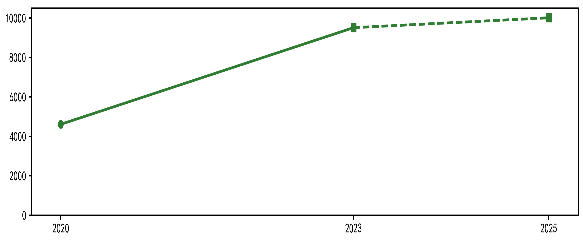
\includegraphics[width=0.8\textwidth]{项目计划书图片/image3.png}
    \caption{东北黑土区保护性耕作面积变化（2020—2025年）}
    \label{fig:2}
\end{figure}

\begin{figure}[htbp]
    \centering
    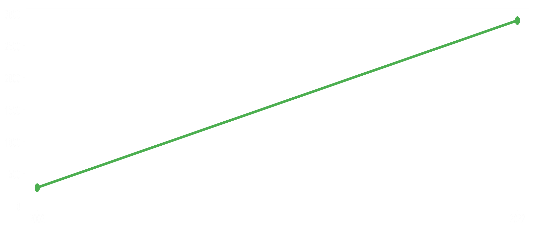
\includegraphics[width=0.8\textwidth]{项目计划书图片/image4.png}
    \caption{东北主要粮食作物调出价值变化（2002—2022年）}
    \label{fig:3}
\end{figure}

\subsection{3.成效与需求：保护成效凸显，精准监测需求升级}

在一系列政策推动下，东北黑土地保护工作已取得阶段性成效。一方面，黑土区保护性耕作面积持续扩大，从2023年到2025年呈现稳步增长态势，免耕少耕等模式得到广泛推广，说明以少扰动、多覆盖为核心的耕作制度正在被基层生产主体接受并落地；另一方面，2002年至2022年间，东北主要粮食作物调出价值从不足500亿元增长至近3000亿元，印证了黑土地保护与粮食产能提升的协同效应，体现了黑土地作为国家粮食安全“压舱石”的关键作用。上述两方面变化相互印证，表明保护性耕作等举措在遏制退化趋势、稳定粮食产能方面已经产生了实际效果。

对上述两项趋势还需作进一步解读。保护性耕作面积的稳步扩大，反映的不只是推广力度的加强，更说明基层生产主体对少扰动、多覆盖耕作方式的主动接受程度在提高。粮食调出价值的持续增长则表明，黑土地在保护措施同步推进的条件下仍能稳定输出大规模商品粮，保护与产能之间并非此消彼长的对立关系。同时也应看到，面积数据主要来源于统计上报，价值变化还会受到市场价格波动等因素影响，二者均不能直接等同于耕地质量的实质改善；要判断有机质是否真正提升、黑土层是否真正增厚，仍须依靠直接观测获取的空间数据加以验证。

与此同时，保护工作的推进也使监测对象趋于复杂：地表覆盖形式更加多样，地块边界与耕作方式处于动态调整之中，退化与恢复过程往往在空间上零散分布、在时间上逐年渐变，仅凭人力与低精度手段难以准确刻画。当前，黑土地保护已进入“依法治土、精准治理”的新阶段，对监测技术的精准性、实时性、低成本性提出了更高要求：既要求能够分辨地块尺度的细微变化，又要求具备足够高的观测频次以捕捉变化过程，还必须把使用成本控制在基层可承受的范围内，否则技术能力难以真正下沉到县域与乡镇一线。

本项目聚焦黑土地保护的精准监测需求，正是为了进一步落实《黑土地保护法》及相关政策要求，通过智能化技术破解传统监测短板，助力实现黑土地“总量不减少、功能不退化、质量有提升、产能可持续”的保护目标，为国家粮食安全提供坚实的科技支撑。

% ==================== 片段 g4 ====================
\section{五、项目痛点——传统监测体系的四大核心短板}

结合黑土地保护的一线调研与行业现状分析，当前黑土地监测治理工作仍面临四大核心痛点，直接制约了保护工作的精准性与高效性。四类短板彼此关联、层层递进，共同构成“看得不全、看不精、看不准、用不起来”的现实困境。

\subsection{1.传统人工监管效率低下}

传统黑土地监管多依赖人工实地巡查方式，整体作业效率低下。人工巡查不仅人力、时间成本高昂，巡查周期偏长、巡查范围有限，存在监管覆盖不全面、巡查盲区多等问题，难以实现黑土区大范围、全天候、常态化的动态监测与全域巡查。从作业组织角度看，一次完整巡查需经历路线规划、现场取证、影像记录、内业整理等环节，高度依赖人员经验。

同时人工排查响应速度慢，数据记录与反馈存在滞后性，无法及时捕捉黑土地侵蚀、地力下降、违规侵占等退化问题，难以满足黑土地保护治理工作中“早发现、早预警、早治理”的核心管控需求。黑土地退化兼具渐变与突变特征：侵蚀沟发育、表土流失在早期多表现为细微的地表纹理变化，人工巡查受限于人眼判别能力与有限的地面视角，很难在变化初始阶段识别；而当退化迹象肉眼可见时，治理成本与修复难度已显著上升。因此，缺少高频次、大范围、可回溯的自动化监测手段，是人工监管模式难以突破的瓶颈。

\subsection{2.传统遥感监测精度不足、成本高昂}

现阶段常规遥感监测技术手段存在明显短板，空间分辨率有限、监测精度不足，易受云层、植被物候、光照环境等外界因素干扰，产生大量伪变化、误判及漏判现象，监测数据可靠性不足。究其机理，中等分辨率影像中单个像元往往混合多种地物光谱，零星退化斑块在像元尺度上被稀释，难以稳定提取；同时同一地块在不同季节与光照条件下的光谱响应本身就会变化，若解译方法不能区分“地表真实改变”与“成像条件改变”，就会引入大量伪变化噪声。

同时，高精度、高分辨率遥感影像数据采购与获取费用昂贵，整体监测投入成本居高不下，难以长期大面积普及应用。对县域、农场等一线保护单元而言，监测经费与人力较为有限，若每次监测都需为数据获取与人工解译支付高昂成本，监测频次必然被迫降低，形成“成本越高、频次越低、数据越旧”的负向循环。该模式难以适配黑土地保护的精细化管理要求，无法开展地块尺度的常态化精准监测，也不能快速识别侵蚀沟发育、水土流失、土壤有机质流失、耕地违规破坏等关键退化问题。

从供给端看，现成的高精度商业遥感解译方案同样难以直接套用。一是通用商业平台多以地物分类、作物长势监测为主营方向，其模型面向地块边界提取与作物类型识别等任务训练，缺少对侵蚀沟、水土流失等退化类型的针对性判别能力，场景迁移后精度衰减明显；二是此类服务通常按影像面积或调用量计费，且需将原始影像上传至厂商云端处理，对数据敏感、经费有限的一线单元而言，成本与数据安全两方面均存顾虑；三是通用平台的输出多为栅格分类结果与统计报表，缺少与地块台账、治理措施相衔接的业务接口，难以嵌入“发现—核实—处置”的一线流程。因此，只有立足本场景自建模型与数据体系，才能形成可负担、可掌控、可落地的专用监测能力。

\subsection{3.深度学习模型泛化能力弱}

现有模型对复杂场景的变化误判率高，难以有效区分真实土地退化与季节性植被变化、光照变化等干扰因素，检测结果可靠性不足，无法直接用于指导治理决策。变化检测的本质是判断同一地块在两个时相之间是否发生了实质性改变，而真实农业遥感场景中，作物轮作、播种收割、土壤翻耕、积雪消融等常规农事活动都会带来显著的地表影像变化，其表现与部分退化现象高度相似；若模型缺乏全局语义建模能力，仅依赖局部纹理与颜色差异判别，就极易将正常农事活动误判为退化。

从模型结构层面看，传统卷积网络\cite{ref5,ref7}受限于固定感受野，特征提取集中于局部邻域，对跨空间范围的地物关联与地块形态变化缺乏感知能力；同时，不同区域的地形地貌与种植结构差异明显，模型在一个区域训练所得的特征分布难以直接迁移到另一区域，跨区域应用时精度衰减明显。这使模型输出仍需大量人工复核才能进入治理流程。如图~\ref{fig:img5}所示，本项目在实测场景中对模型误判问题进行了针对性分析验证。

\begin{figure}[htbp]
    \centering
    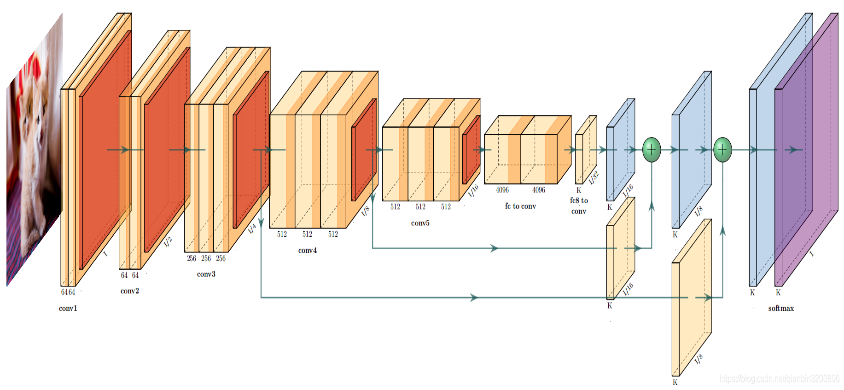
\includegraphics[width=0.8\textwidth]{项目计划书图片/image5.png}
    \caption{现有深度学习模型在复杂场景下的变化误判效果示意}
    \label{fig:img5}
\end{figure}

\subsection{4.数据应用脱节，难以形成治理闭环}

当前黑土地保护各类多源监测数据分散存储、独立管理，部门之间数据共享不畅，普遍存在信息孤岛现象。卫星影像、无人机航拍、地面采样、农事记录等数据往往由不同主体按各自业务需要分别采集保存，在格式规范、坐标基准、时间粒度、属性字段等方面缺乏统一约定，即便同一区域的数据也难以直接叠加使用，数据流通成本高、时效性差。

各类监测数据缺乏标准化整合、统一管理与深度融合，缺少一体化、智能化的综合决策支撑平台。海量监测成果得不到有效挖掘与利用，无法快速转化为科学、可落地的治理决策依据，数据价值难以释放。整体业务链条割裂断层，无法打通“实时监测—智能预警—精准施策—长效治理”的全流程衔接，难以形成完整、高效的管控治理闭环，大幅降低黑土地保护与修复工作的推进效率。若不能以统一平台为纽带，将数据采集、解译、预警与处置串联为可追溯、可反馈的完整链路，再先进的算法也难以作用于田间地头的治理实践。

上述四大痛点并非彼此孤立，而是存在清晰的因果传导关系：监测手段的效率不足，迫使基层以低频次、小范围的人工巡查替代常态化监测，造成问题发现滞后；发现滞后又使监测数据在时间维度上残缺，样本难以覆盖退化过程的完整阶段，真值质量不足，模型泛化能力随之受限；而精度不足的检测结果无法直接进入治理流程，必须依赖人工复核，反过来进一步加重人力负担；分散的数据与低可信度的结果彼此叠加，最终使监测成果难以转化为治理决策。由此看，效率问题抬高了监测的成本下限，精度问题限制了监测的可信上限，也决定了本项目必须同时从算法与系统两侧入手，而非单点优化。

\section{六、项目设计思路}

针对传统黑土地监测方案的四大痛点，本项目从模型、数据、系统架构三个维度出发，构建了一套高效、精准、可落地的技术方案：以算法优化解决“看不准”，以专用数据集解决“数据不适用”，以轻量化架构解决“用不起来”。

\subsection{1.模型优化：轻量化、高精度的变化检测算法}

本项目以改进的ResNet18作为backbone提取高分辨率影像特征，结合轻量化语义分词器与BIT双时相Transformer模型，捕捉全局时空语义信息；同时支持与传统模型灵活切换，构建了一套高效、精准的黑土地变化检测系统，有效解决了现有模型误判率高、泛化能力弱的问题。

在技术原理上，模型采用双分支结构分别编码前后两个时相影像：卷积骨干网络提取局部纹理与边界特征，语义分词器将特征图映射为具有语义含义的语义tokens，使局部特征被组织为可交互的语义单元；随后由BIT双时相Transformer在两组语义tokens之间进行全局注意力计算，在整幅影像范围内判断“哪些语义单元发生了变化”，从而有效区分真实退化与季节性植被变化、光照差异等干扰。该设计同时控制参数量与计算开销，配合批量化推理策略，使模型在普通算力条件下即可完成批量推理，识别精确率达到70\%、算力成本降低69\%，为周级高频监测提供了可行的算力基础。

需要说明的是，模型轻量化与检测精度之间并非简单的此消彼长。本项目所做的取舍，是以结构性的改进换取参数效率，而非以牺牲精度为代价压缩模型规模：ResNet18作为骨干网络参数量适中、特征提取稳定，契合亚米级影像中耕地边界、侵蚀沟等目标的外观特征；语义分词器在降低特征图空间规模的同时保留语义单元之间的对应关系，使全局注意力计算的开销随影像尺寸增长更为平缓；BIT双时相Transformer则把算力集中投入到“变化”这一关键任务上，避免在无变化的背景区域重复计算。三者叠加，使模型在普通算力条件下仍能完成整幅影像的推理，从而支撑周级高频监测所需的吞吐能力。

\subsection{2.数据支撑：构建黑土地专用遥感数据集}

项目构建了覆盖多种退化类型的黑土地专用遥感数据集，采用ArcGIS专业标注保证真值可靠；数据集兼容卫星（如GF-2）与无人机等多源光学影像，贴合实际监测场景的数据源特性，为模型训练与系统运行提供了高质量的数据支撑。

数据集建设围绕“覆盖全面、标注规范、来源多元”三个目标展开。覆盖范围上，样本涵盖侵蚀沟发育、水土流失、土壤有机质流失、耕地违规破坏等典型退化类型，并纳入正常农事活动引起的地表变化作为负样本，使模型学习真实退化与干扰变化之间的判别边界；标注规范上，依托ArcGIS平台进行矢量勾绘与属性录入，统一坐标基准与类别定义，并通过交叉复核控制标注误差；数据来源上，同时纳入国产高分二号亚米级卫星影像与无人机航拍影像，兼顾大范围覆盖与局部高精度细节，提升真实业务场景中的泛化能力。

专用数据集对精度提升的作用，主要体现在降低“语义歧义”与“场景偏差”两个方面。其一，退化现象在影像上多表现为纹理、色调、边缘形态等弱特征，若训练样本中缺少同类案例，模型只能依据表面相似性进行判别，容易把翻耕、收割等常规农事活动误判为退化；引入负样本后，模型得以学习到“发生了变化但并非退化”的判别边界，误判随之减少。其二，跨区域应用时的精度衰减，主要源于训练分布与目标区域的地形地貌、种植结构不匹配，而多源样本与统一标注规范的结合，使特征分布的覆盖范围更广，迁移到新区域时更稳定。可见数据集的覆盖度与标注质量，直接决定了模型精度所能达到的上限。

\subsection{3.系统架构：前后端分离的轻量化部署方案}

系统采用前后端分离的轻量化架构：后端以FastAPI支撑高性能批量处理，前端提供简洁易用的可视化界面，普通电脑即可本地化部署运行，有效降低了一线用户的使用门槛，解决了传统方案“数据应用脱节、难以形成闭环治理”的痛点。

前端可视化Web系统围绕一线业务人员的实际使用路径设计，集成影像上传、变化检测、结果可视化、AI解读与一键报告等核心功能：用户上传前后时相影像后可在线发起检测任务，结果以图层叠加、变化斑块高亮等方式直观呈现，并可通过AI解读模块获得对变化成因与影响的中文说明，最终一键生成结构化报告。后端采用模块化服务设计，将影像预处理、模型推理与报告生成解耦为独立服务，便于按需扩展算力与升级模型；前后端以标准接口通信，使系统可在普通配置计算机上完成本地化部署，将智能监测能力下沉到县域、农场等一线单元，形成“上传—检测—解读—报告—处置”的完整业务闭环。

% ==================== 片段 g5 ====================
\section{七、项目技术的支撑}

\subsection{1.监测技术升级的现实需求}

黑土地是保障国家粮食安全的重要战略资源，其退化过程具有缓变、隐蔽、空间异质性强等特点，只有依靠高频次、高精度、可重复的观测手段，才能及时捕捉退化趋势并支撑保护性耕作决策。长期以来，东北黑土区的监测工作主要依赖传统手段，与常态化、精细化的保护需求之间存在明显差距，具体表现为以下几个方面。

\begin{itemize}
    \item \textbf{人工巡查效率低、覆盖范围有限。}以人工实地采样与巡田为主的方式，受人力、车辆、道路条件与作业季节的制约，单次可覆盖的面积十分有限，难以在作物生长关键期内完成大范围同步普查；同时，人工观测结果依赖经验判断，不同人员在判读口径上难以完全统一，数据的可比性与可追溯性不足。
    \item \textbf{常规卫星遥感分辨率不足。}中低分辨率遥感产品虽然具备大范围覆盖能力，但其像元尺寸往往大于田间地块的实际尺度，混合像元效应显著，难以识别地块尺度的退化细节，如侵蚀沟发育、耕作层变薄、地表裸露程度变化等，往往只能反映区域平均状态，无法支撑逐地块的差异化管理。
    \item \textbf{国外高分辨率数据获取成本高、周期长。}国外亚米级遥感数据在采购费用、重访安排与数据交付环节均存在较多限制，成本与周期难以匹配常态化监测的需要，且数据获取的稳定性与连续性存在不确定性，不利于形成长时序、可对比的监测档案。
\end{itemize}

综合以上短板可以看出，黑土地保护工作迫切需要一套\textbf{国产化、高精度、大范围}的遥感监测方案：以自主可控的数据源为基础，摆脱对外部数据供给的依赖；以亚米级成像能力为支撑，将观测尺度下沉到地块级；以稳定的重访与交付节奏为保障，形成可持续运行的数据链条，从而为黑土地保护提供稳定、可靠的数据支撑。本项目选择国产高分二号卫星作为主数据源，正是基于上述需求做出的技术判断。

\subsection{2.GF-2卫星的核心技术优势}

高分二号（GF-2）卫星是我国自主研发的首颗亚米级民用光学遥感卫星，专为高分辨率对地观测设计，其技术参数与本项目的监测需求高度契合：一方面，其空间分辨率足以支撑地块尺度的地物判读；另一方面，其幅宽与重访能力可以满足区域尺度的周期性覆盖要求。两者结合，使“既看得清、又看得全、还看得勤”成为可能。

从监测需求出发，GF-2的关键技术参数与本项目形成逐条对应的支撑关系：空间分辨率对应识别精度需求，决定地块边界与侵蚀沟能否被分辨；成像幅宽对应覆盖效率需求，决定区域尺度监测所需的成像次数；轨道与重访能力对应时间频次需求，支撑“周级”动态监测持续运行；载荷成熟度与产品供给稳定性对应工程可靠需求，决定长期业务化运行的风险水平。上述参数与数据保障条件彼此配合，共同支撑起从影像获取到变化检测的完整链路。表~\ref{tab:gf2}汇总了 GF-2 的主要技术参数及其对本项目的支撑作用。

\begin{table}[htbp]
    \centering
    \caption{高分二号（GF-2）卫星主要技术参数及其对本项目的支撑}
    \label{tab:gf2}
    \small
    \begin{tabular}{|p{2.6cm}|p{5.6cm}|p{5.8cm}|}
        \hline
        \textbf{参数类别} & \textbf{技术指标} & \textbf{对本项目的支撑作用} \\
        \hline
        发射与轨道 & 2014 年 8 月 19 日发射；太阳同步回归轨道，轨道高度 631 km，回归周期 69 天 & 成像光照条件稳定、重访规律，保障多时相影像可比 \\
        \hline
        空间分辨率 & 星下点全色 0.8 m、多光谱 3.2 m & 亚米级成像可清晰分辨地块边界、植被覆盖度与侵蚀沟等细部特征 \\
        \hline
        成像幅宽 & 45 km（两台相机组合） & 单景覆盖范围大，减少区域监测所需的影像拼接与重访次数 \\
        \hline
        侧摆与重访 & 侧摆能力 $\pm35^\circ$，侧摆条件下重访周期约 5 天 & 支撑“周级”动态监测的频次要求 \\
        \hline
        载荷谱段 & 全色 0.45--0.90 $\mu$m；多光谱：蓝 0.45--0.52、绿 0.52--0.59、红 0.63--0.69、近红外 0.77--0.89 $\mu$m & 覆盖植被与土壤诊断光谱区间，支持植被指数计算与地力指标反演 \\
        \hline
        定位精度 & 无地面控制点时约 50 m（CE90） & 保障多时相影像几何配准精度，减少配准误差引起的伪变化 \\
        \hline
        数据供给 & 国产民用高分辨率卫星，产品成熟稳定 & 数据来源自主可控，保障长时序监测档案的连续性 \\
        \hline
    \end{tabular}
    \par\vspace{2pt}
    {\footnotesize 注：表中参数依据高分二号卫星官方公布数据整理。}
\end{table}

\begin{figure}[htbp]
    \centering
    
\includegraphics[width=0.8\textwidth]{项目计划书图片/image6.png}
    \caption{高分二号（GF-2）卫星技术参数说明（一）}
    \label{fig:4a}
\end{figure}

\begin{figure}[htbp]
    \centering
    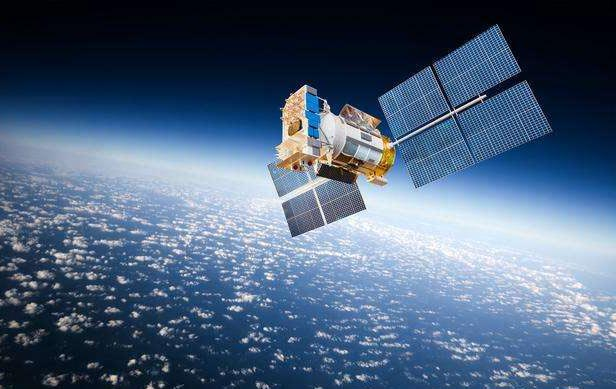
\includegraphics[width=0.8\textwidth]{项目计划书图片/image7.jpeg}
    \caption{高分二号（GF-2）卫星技术参数说明（二）}
    \label{fig:4b}
\end{figure}

\subsubsection{（1）空间分辨率：从“看得见”到“看得清”}

全色波段分辨率达0.8米，多光谱波段分辨率为3.2米，属于亚米级高清成像水平。这一分辨率水平意味着单个像元对应的地面尺寸小于一米，已明显优于田间常见地物的尺度阈值：地块边界、田埂与道路走向在影像上可清晰分辨，植被覆盖度的疏密差异可通过纹理与光谱组合加以区分，侵蚀沟等线状微地貌也能被有效识别。对于黑土地精细化监测而言，空间分辨率直接决定了退化指标能否被观测到——只有将观测尺度下沉至地块一级，才能对黑土区地块边界、植被覆盖度、侵蚀沟等细微地物特征进行稳定判读，进而满足黑土地精细化监测的精度要求。全色与多光谱的波段组合，则在保证几何细节的同时保留了地物光谱信息，为后续变化检测模型提供了信息量更充分的数据基础。

亚米级分辨率的价值，在地块边界与侵蚀沟两类目标上体现得尤为直接。地块边界多由田埂、道路、沟渠等窄线状地物构成，宽度往往不足数米，在中低分辨率影像上极易被混合像元淹没，而在高分辨率影像上则呈现为连续清晰的线状特征，使地块几何轮廓得以准确勾画，这是开展逐地块统计与差异化管理的前提。侵蚀沟属于典型的缓变型线状微地貌，发育初期宽度较小、与周边耕地光谱差异有限，只有在足够精细的空间尺度上才能被稳定识别；将其纳入常态化监测对象，有助于在沟蚀尚处初期时发现问题，避免其扩展造成耕作层不可逆损失。

\subsubsection{（2）成像幅宽：从“看得清”到“看得全”}

单次成像幅宽达45公里，可实现大面积区域的同步覆盖。幅宽是决定监测效率的关键参数：幅宽越大，单轨可覆盖的地面范围越广，拼接与配准的工作量越小，同一时相内影像的辐射与几何一致性也越好。相较于幅宽偏窄的高分辨率卫星，GF-2能够在更少的成像次数内完成同等面积的观测，成像效率远超国外同类卫星。这一特性与松嫩平原等黑土集中连片分布区的空间形态高度匹配，能够高效完成东北黑土区大范围、周期性的动态监测任务，为“周级”动态监测的频次目标提供了工程上可行的时间余量。

\subsubsection{（3）轨道与成像能力：从“看得全”到“看得懂”}

卫星采用太阳同步轨道，轨道高度约631公里，可稳定获取高重访率的观测数据。太阳同步轨道使卫星在相近的地方时过境，成像时的太阳高度角与光照条件相对一致，不同时相影像之间的光照差异被显著压缩，有利于开展多时相对比与变化检测——这一点对双时相模型尤为重要，因为光照与物候差异是造成伪变化的常见来源。

在载荷配置上，卫星搭载蓝、绿、红、近红外四波段多光谱传感器。多光谱信息是地物属性反演的基础：可见光波段反映地表反射特性与植被绿度状况，近红外波段对植被长势与含水量高度敏感。依托这些波段，可通过光谱特征反演土壤有机质含量、作物长势、土壤湿度等关键指标，并结合植被指数等成熟方法增强对地表覆盖状态的判别能力，从而为黑土地质量评估提供多维度数据，使变化检测结果不仅有“变了多少”的空间信息，也具备“为什么变、变得好不好”的属性解释空间。

在具体的地力指标反演层面，四个波段可组合出多种成熟的光谱指数与反演思路：以近红外与红光构建的植被指数可表征作物长势与植被覆盖度，进而反映耕地利用强度与地表裸露程度的变化；可见光波段组合有助于区分裸土、秸秆残茬与绿色植被，为保护性耕作中秸秆覆盖状况的判读提供依据；近红外波段对水分吸收的敏感性，可用于推断土壤表层湿度与作物受旱程度。将光谱反演结果与变化检测得到的空间图斑叠加分析，可把“哪里发生了变化”与“变成了什么状态”对应起来，为有机质下降、水土流失等退化判断提供更完整的证据链。

\subsubsection{（4）成熟度与可靠性：从“用得上”到“用得稳”}

该卫星技术路线获国家重点研发计划支持，已在国土资源调查、农业遥感、生态监测等领域得到广泛应用与官方认可，数据产品成熟度高、稳定性强。对项目而言，选择成熟卫星数据源的意义在于降低不确定性：数据格式规范、几何与辐射处理流程完善、产品供给稳定，可以使研发资源更多集中于变化检测算法与业务系统本身，而无需在数据获取与预处理环节反复适配。稳定的数据供给也保证了长时序监测档案的连续性，为本项目2026年落地试点、2028年推广至黑吉辽蒙四省区乃至2030年构建“天空地”一体化监测网的分阶段目标，提供了可靠的技术保障。

\subsubsection{（5）数据自主可控：从“用得上”到“用得久”}

选择国产卫星数据源，还基于数据安全与供应链自主可控的现实考量。高分辨率遥感影像的采集、存储、传输与处理涉及大量地理空间信息，其获取渠道、交付周期与使用条件若受制于外部因素，将影响监测工作的连续性与长时序数据口径的一致。采用自主可控的国产卫星数据，一方面可避免采购与授权环节的不确定性，使数据获取节奏与项目推进节奏相匹配；另一方面，国产数据产品的格式规范、坐标基准与处理工具链在国内具有更好的适配基础，便于与既有地理信息平台对接，也便于在本地化部署环境中完成数据处理，降低对外部服务依赖带来的运行风险。对面向黑土地保护的长期监测任务而言，这种稳定、可持续的数据保障能力，与算法能力和系统能力同等重要。

% ==================== 片段 g6 ====================
\section{八、产品设计——模型、数据与系统三位一体}

本项目以 BIT 检测模型与专用遥感数据集为核心基础，结合轻量化 Web 前端系统，构建了一套完整的耕地变化监测产品。算法模型解决“看得准”的问题，专用数据集解决“学得会”的问题，可视化前端解决“用得上”的问题，三者协同支撑，具体设计如下。

\subsection{1.核心算法：BIT模型框架}

模型以改进的 ResNet18为 CNN 骨干网络，对双时相输入影像进行特征提取，再通过语义分词器与双时序图像转换器，利用 Transformer 编码器捕捉全局时空上下文信息；最后通过解码器输出精细特征，经预测头生成最终的变化检测结果图，实现了高精度、低误判的黑土地变化检测。

从数据流看，该框架可分为四个阶段：T1、T2两个时刻的影像分别进入共享权重的 ResNet18骨干网络，得到两组空间分辨率逐级降低、通道数逐级增加的中间特征图；语义分词器对特征图做语义级压缩，将其转化为数量可控的语义 token 序列；Transformer 编码器对两个时相的 token 序列进行跨时相交互，借助自注意力在整幅影像范围内建立长程依赖，使同一空间位置在两个时刻的语义特征得以直接比对；解码器再逐级上采样恢复空间分辨率，由预测头输出逐像素的变化概率图。卷积结构与自注意力机制在此形成互补：前者适配遥感影像的局部纹理与边缘特征，后者不受卷积核感受野限制，对形状不规则、分布零散的变化斑块更具判别力，有助于在复杂地表背景下抑制伪变化。项目采用 BIT（Bipartite Transformer）模型\cite{ref1,ref8}作为核心算法，整体框架如下图所示。

四个阶段中，共享权重设计是可比性的前提：两个时相经同一套卷积参数映射到同一特征空间，同一位置的响应才具有统一尺度，否则特征分布出现整体偏移，比对便失去基准。语义分词器承担语义归纳职责，把特征图上数量庞大的空间位置压缩为数量固定的语义 token，每个 token 对应影像中一类语义一致的区域。跨时相交互是判别力的主要来源：编码器把两个时相的 token 序列置于同一注意力计算中，每个 token 都可查询另一时相中语义相近的 token 并交换信息，从而在整幅影像范围内建立长程依赖。解码器再逐级上采样把结论还原到像素级，由预测头输出逐像素的变化概率。

与传统的单时相差分方法相比，双时相交互设计的优势体现在三个方面。其一，差分法直接比较两个时相的像素灰度，对配准误差、光照差异十分敏感，农田翻耕、作物收割等物候现象容易被误判为地表覆盖改变；双时相交互在特征空间中比对语义，学到的是地类是否发生实质改变，对同物异谱、同谱异物现象更为鲁棒。其二，差分法通常只能给出变化与否的二值结论，而跨时相注意力保留了两期影像之间的语义对应关系，可为按类型统计变化面积提供依据。其三，差分阈值需针对不同区域与季节人工标定，迁移到新区域时须重新调参；改进 BIT 的判别边界由数据驱动学习得到，更换监测区域时补充少量样本即可适配。

\begin{figure}[htbp]
    \centering
    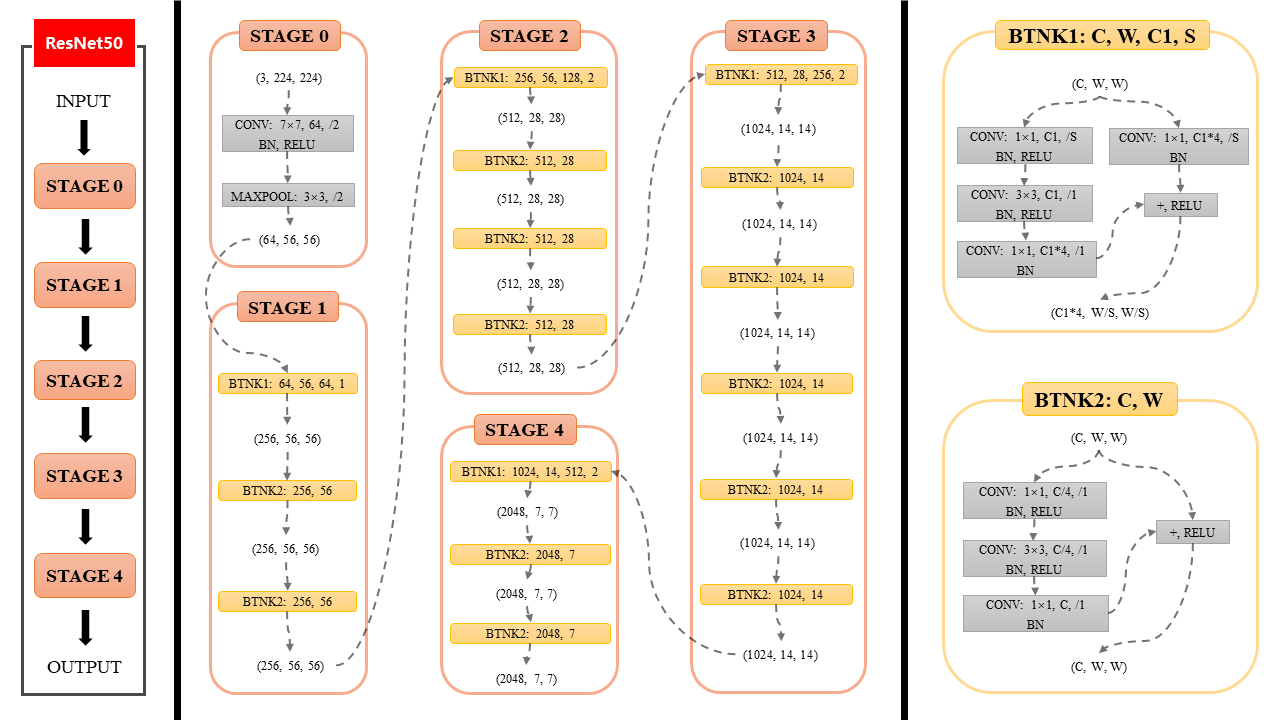
\includegraphics[width=0.8\textwidth]{项目计划书图片/image9.png}
    \caption{ResNet 骨干网络结构拓扑图}
    \label{fig:5}
\end{figure}

\begin{figure}[htbp]
    \centering
    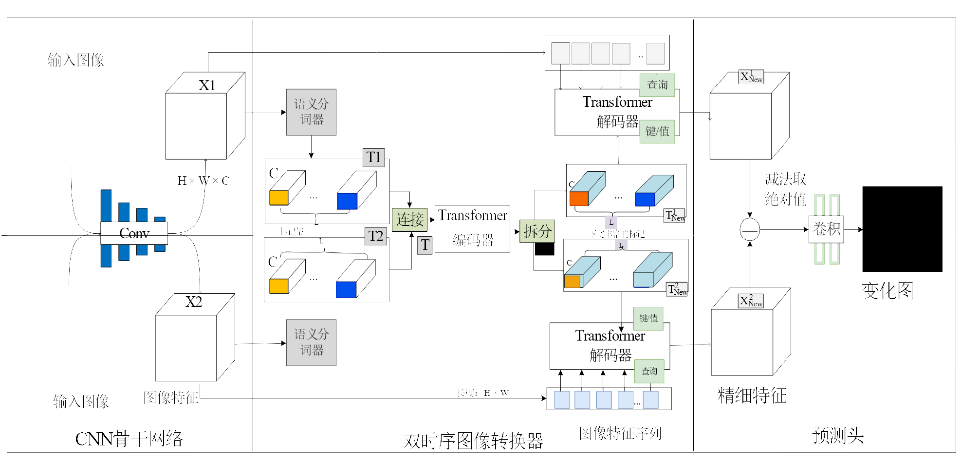
\includegraphics[width=0.8\textwidth]{项目计划书图片/image10.png}
    \caption{BIT模型框架}
    \label{fig:6}
\end{figure}

语义分词器用于从图像特征中提取语义 tokens，配合 Transformer 做图像任务。若把每个空间位置的特征都视为一个 token，注意力计算量将随影像分辨率急剧增长，难以在普通设备上完成推理；语义分词器即在于进入 Transformer 之前完成一次语义压缩，用少量语义明确的 token 概括整幅特征图的信息。

\begin{figure}[htbp]
    \centering
    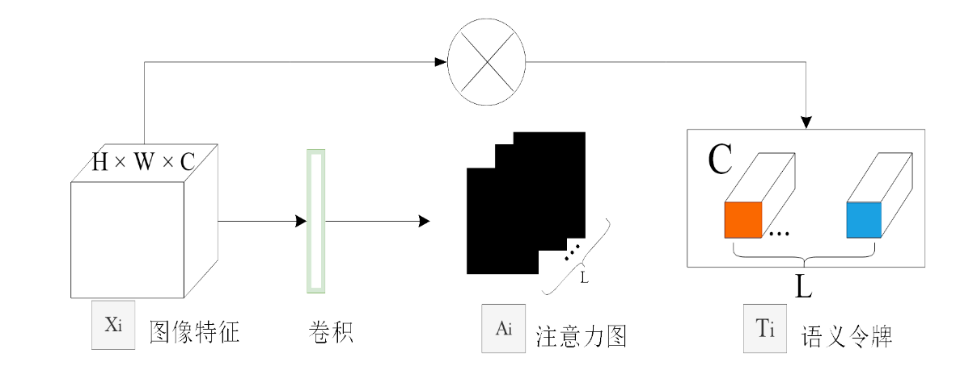
\includegraphics[width=0.8\textwidth]{项目计划书图片/image11.png}
    \caption{语义分词器子模块流程图}
    \label{fig:7}
\end{figure}

其中，语义分词器的核心流程如下：

\begin{enumerate}
    \item \textbf{图像特征输入。}输入是维度为 $H \times W \times C$ 的特征图（$H$ 为高度、$W$ 为宽度、$C$ 为通道数），来自 CNN 骨干网络提取的中间特征。
    \item \textbf{卷积降维与特征变换。}用卷积层对特征图进行处理，目的是降维与特征变换，将其映射到适合度量语义相似性的表征空间，为生成注意力图做准备。
    \item \textbf{生成注意力图。}卷积输出经进一步处理得到 $L$ 张注意力图，每张关注特征图中不同的语义区域，用于捕捉关键语义信息，卷积计算过程如图所示。
    \item \textbf{加权聚合得到语义 token。}以注意力图作为空间权重对特征图加权求和，得到 $L$ 个语义 token；其数量与影像分辨率无关，因而在保证语义完整性的同时压缩了后续计算规模。
\end{enumerate}

语义分词器与自注意力机制之间是“先归纳、后关联”的分工：分词器把空间连续、语义一致的区域聚合成少量 token，自注意力则在这些 token 之间建立全局联系。这一分工使注意力计算规模由与像素数相关转为与 token 数相关，而 token 数量可预先设定且不随影像尺寸增长，因此模型面对亚米级高分影像时仍能把显存占用与推理时间控制在可接受范围。注意力图还带来了可解释性：一张注意力图对应影像中一片被模型重点关注的空间区域，多张注意力图叠加后，可以观察模型在判定“发生变化”时关注了哪些位置，为复核人员排查误判提供线索。

\begin{figure}[htbp]
    \centering
    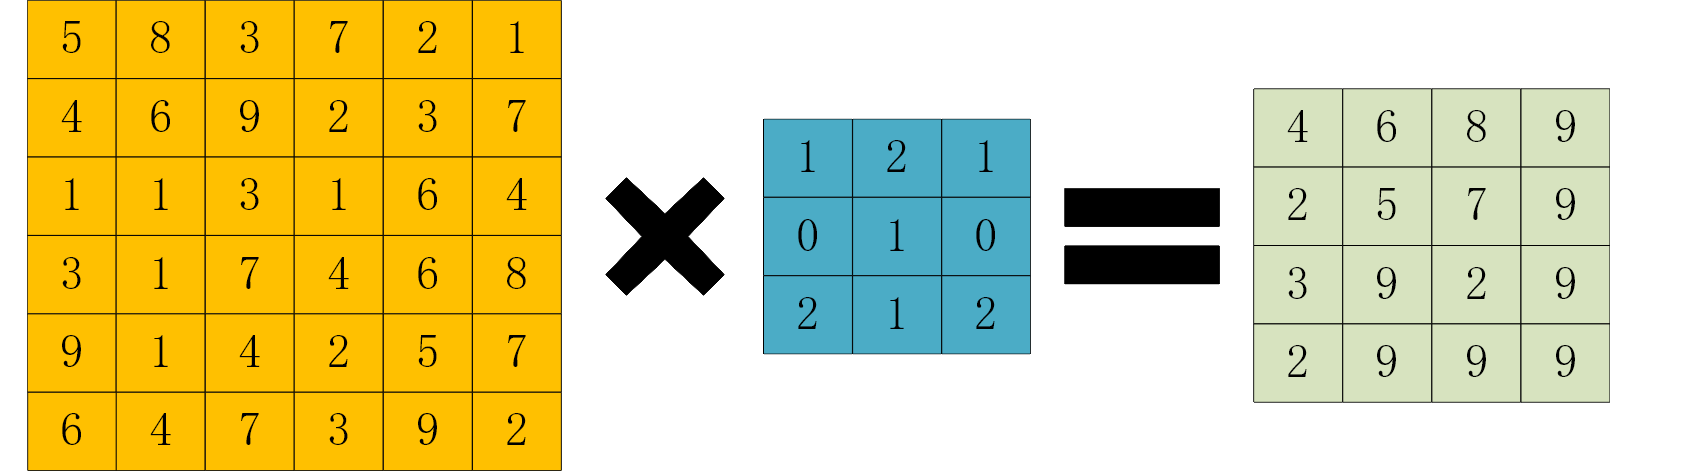
\includegraphics[width=0.8\textwidth]{项目计划书图片/image12.png}
    \caption{卷积计算}
    \label{fig:8}
\end{figure}

该设计使模型在保持识别精度的同时具备良好的推理效率：整体算力成本降低69\%，监测周期缩短33\%，识别精确率达到70\%，为“周级”动态监测提供了算力可行性。

\subsection{2.数据支撑}

算法能力必须建立在高质量数据基础之上。项目构建了黑土地专用遥感数据集，样本以国产高分二号（GF-2）亚米级光学遥感卫星影像为主，辅以无人机航拍影像，覆盖不同季节与地表覆盖类型，以增强模型对真实业务场景的适应能力。表~\ref{tab:dataset}给出该数据集的样本构成。

\begin{table}[htbp]
    \centering
    \caption{黑土地耕地变化检测双时相遥感数据集样本}
    \label{tab:dataset}
    \small
    \begin{tabular}{|c|c|c|c|}
        \hline
        类型 & 时间为T1 & 时间为T2 & 标签 \\
        \hline
        土地变化 & 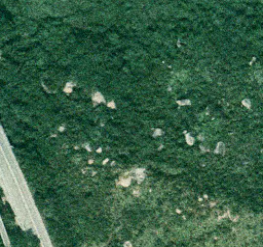
\includegraphics[width=2.4cm]{项目计划书图片/image13.png} & 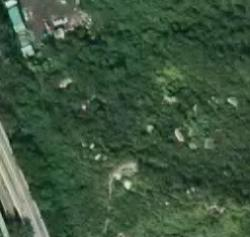
\includegraphics[width=2.4cm]{项目计划书图片/image14.jpeg} & 
\includegraphics[width=2.4cm]{项目计划书图片/image15.png} \\
        \hline
        海上建设 & 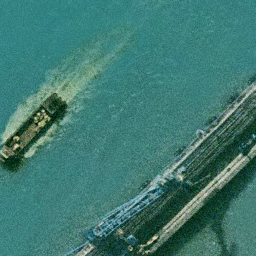
\includegraphics[width=2.4cm]{项目计划书图片/image16.png} & 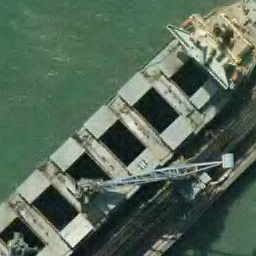
\includegraphics[width=2.4cm]{项目计划书图片/image17.png} & 
\includegraphics[width=2.4cm]{项目计划书图片/image18.png} \\
        \hline
        城市建筑 & 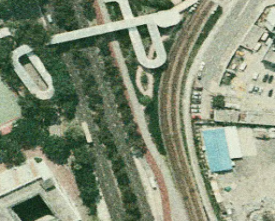
\includegraphics[width=2.4cm]{项目计划书图片/image19.png} & 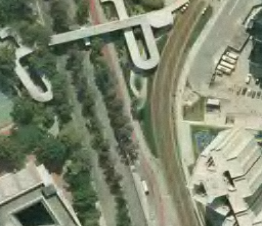
\includegraphics[width=2.4cm]{项目计划书图片/image20.png} & 
\includegraphics[width=2.4cm]{项目计划书图片/image21.png} \\
        \hline
        森林变化 & 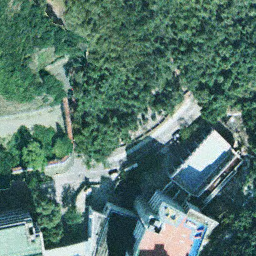
\includegraphics[width=2.4cm]{项目计划书图片/image22.png} & 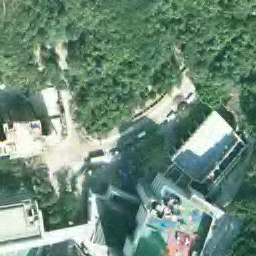
\includegraphics[width=2.4cm]{项目计划书图片/image23.png} & 
\includegraphics[width=2.4cm]{项目计划书图片/image24.png} \\
        \hline
    \end{tabular}
\end{table}

数据集构建遵循“采集—配准—标注—核验”的规范化流程：先选取时间基线一致、云覆盖较少、影像质量合格的 T1、T2影像对，完成几何配准与辐射归一化，使两个时相一致对应，排除成像条件差异造成的伪变化；再用 ArcGIS 等专业工具人工标注，逐像素勾绘变化区域边界，形成与影像对一一对应的真值标签；最后通过交叉复核与抽样检查把关质量，对边界模糊、地类易混淆的样本复判或剔除，保证真值可靠性。样本覆盖土地变化、海上建设、城市建筑、森林变化等场景：土地变化样本直接对应耕地被占用、撂荒等地表覆盖改变；海上建设、城市建筑等强变化样本有助于区分真实变化与季节性物候波动；森林变化样本则提升对植被类地物的判别能力。多类型混合训练使模型学习“地表发生变化”的共性规律而非某类地物的外观特征，从而对未见过的变化形态保持泛化能力。

尤需说明的是，数据集的价值不仅在于样本数量，更在于场景分布的代表性。变化检测模型在训练中容易走“捷径”，依据地物外观而非变化本身作出判断，例如把偏绿的影像一律归为植被、把规则矩形一律归为建筑，一旦遇到训练集中未出现的组合便会失效。为此，数据集在构建时有意拉大场景类型的跨度：既包含农田转为建设用地的渐变型变化，也包含地表裸露、水体外扩等突变型变化；既覆盖成片连续的变化，也保留分散、边界不规则的细碎变化。不同类型样本相互约束，迫使模型把判别依据收敛到“两个时刻之间究竟发生了什么”这一核心问题上，以场景覆盖换取对新区域、新变化形态的泛化能力。

需要说明的是，上述场景样本承担的是“通用变化判别”训练任务，其类别设置着眼于覆盖多样的地表变化形态；而黑土地保护业务真正关注的目标类别——侵蚀沟发育、水土流失、土壤有机质流失、耕地违规破坏等——则通过专用样本进行场景适配。二者构成“通用预训练 + 场景适配”的两级训练策略：前者使模型具备对地表变化的通用敏感性，后者把这种敏感性收敛到黑土地退化的具体业务口径上，避免模型把判别依据绑定在某一类地物的外观特征上。

\subsection{3.系统落地：可视化智能前端}

基于前后端分离的轻量化架构，项目开发了一套集影像上传、变化检测、结果可视化、AI 智能解读于一体的现代化遥感检测 Web 前端系统。后端采用 FastAPI 承载模型推理与业务逻辑，前端负责交互呈现，两部分通过标准接口通信，既保证推理服务的稳定性，也便于界面与算法版本的独立迭代。

前后端分离的架构选择同样出于实用考量。算法模型对运行环境存在依赖，若与界面代码耦合，界面调整就可能牵动推理服务重新部署；把推理与呈现拆分为两个独立进程后，模型迭代与前端迭代互不干扰，也便于在不同算力条件的设备上分别优化。

系统支持单张/批量影像上传与处理，自动生成变化检测结果图、热力图与变化比例统计，同时提供一键生成分析报告的功能。单张检测面向定点核查与个案复核，上传一对双时相影像即可获得即时结果；批量检测面向区域性周期性普查，可一次性提交多组影像并统一输出结果与统计汇总，减少人工逐幅操作的工作量。可视化环节给出三类互补信息：结果图以颜色叠加直观标出变化区域的位置与范围；热力图以概率强度反映模型判定的置信程度，帮助区分确定性较高的变化与需人工复核的疑似变化；变化比例统计以结构化方式汇总变化面积占比，为黑土地保护成效评估提供量化依据。AI 智能解读可将像素级输出转译为基层人员易于理解的自然语言描述，一键生成分析报告则将影像、结果图、统计指标与文字解读整合为规范文档，实现从数据输入到决策支撑的全流程闭环。系统面向普通电脑设计，无需专用服务器与高性能显卡即可本地化部署运行，配合算力成本降低69\%、监测周期缩短33\% 的算法优势，降低了一线用户的使用门槛。

前端功能划分遵循“任务—信息—决策”三层递进的取舍原则。任务层只保留影像上传与检测触发两类操作，把参数配置收敛为少量默认项，使不具备遥感背景的基层人员也能独立完成一次检测；信息层在结果图上叠加变化区域、热力图与统计图表，分别回答变化在哪里、模型有多确信、总体变化了多少三个问题；决策层把上述要素汇聚为可下载的分析报告，使检测结果直接进入工作记录与上报流程。单张与批量检测则是两条并列路径：前者面向定点核查，强调上传即得结果，后者面向周期性普查，强调一次提交、统一输出。

\subsection{4.灾害定损模块：从变化检测到经济损失测算}

变化检测回答“哪里变了”，而基层管理者与保险机构真正需要回答的是“损失多大”。二者之间隔着一层换算，项目在这一层的处理原则是：把系统能算出来的，与只能由人给定的，严格分开。

灾害定损模块以已有的双时相检测记录为输入，读取模型输出的变化置信度概率图与变化掩膜，将变化像素按置信度高低划分为轻度、中度、重度、绝收四个等级，等级判定边界可由使用者按当地实际调整。各级受灾面积由该等级像素数占全部变化像素的比例，摊派至使用者填写的地块总面积，从而把像素尺度的检测结果换算为“亩”一级的业务量纲。

经济损失估算遵循“面积×亩产×单价×减产比例”的结构，逐级计算后累加得到总损失估算值。此处必须明确：模型输出的置信度刻画的是影像上发生变化的确定程度，并非实测减产率，二者之间尚无经过标定的换算关系。因此模块并不宣称给出“真实损失”，而是把置信度作为变化强度的代理指标，并将亩产、单价、减产比例等参数全部呈现为可编辑的假设值，由使用者按当地统计年鉴或保险条款替换。测算结果、页面展示与导出文件中一并列出本次采用的全部假设参数及其来源说明，避免假设被误读为测算结论。

模块同时提供查勘成本对比，将人工实地踏勘与遥感辅助定损在单位面积成本与作业周期上的差异并列呈现，使技术替代带来的效益以金额形式直观可见。定损说明文字由大语言模型依据上述已算出的数值生成，该模型不接收任何影像数据，仅对数值作文字组织，且输出结果被明确标注为待复核草稿。如此设计的原因在于，定损结论一旦进入业务记录便具有事实效力，系统因此在流程上始终把最终判断交还给人工核验。

综上，模型、数据与系统三者的协同设计，使项目形成了从算法可研到工程可用的完整链路，共同支撑“天空地一体化光学遥感采集 + AI 智能解译 +可视化决策支撑”的业务闭环，服务于黑龙江松嫩平原试点区域的“周级”动态监测需求，并已在松嫩平原试点中服务500+农户、覆盖10万亩黑土地、支撑新增智能监测岗位30+。

% ==================== 片段 g7 ====================
\section{九、项目落地——面向一线的可推广智能监测方案}

本项目已在黑龙江松嫩平原开展试点应用，形成了成熟的落地模式，面向黑土地保护一线，提供“装得起、用得上、测得准”的智能监测工具：“装得起”指硬件门槛足够低，“用得上”指基层人员无需遥感专业背景即可独立操作，“测得准”指真实业务场景下识别结果稳定可靠，三者共同构成项目从技术成果走向一线生产力的闭环。

\subsection{1.试点区域与成效}

项目以黑龙江松嫩平原为试点区域，实现了耕地变化的“周级”动态监测，能够精准识别撂荒、非法占用、侵蚀沟扩展等关键黑土地退化类型，为基层土地管理提供了及时、可靠的决策依据。

松嫩平原地处东北黑土区核心地带，耕地连片规整，既便于卫星影像解译结果与地面核查逐块比对，也覆盖了较为集中的黑土地退化问题，能够使算法在真实的下垫面条件下得到充分检验。在监测频次上，项目改变了以往依赖人工实地巡查、成果按年度更新的作业方式，转为“周级”动态监测，所针对的是两类不同的变化规律：非法占用等行为具有突发性和隐蔽性，一旦错过发现窗口，后续取证与整改成本将显著上升；撂荒与侵蚀沟扩展变化相对缓慢，需要长时间序列的连续观测才能判断其趋势。项目采用的改进 BIT 双时相 Transformer 模型以语义分词器提取语义 tokens，在双时相影像之间建立长程语义对应关系，可对不同尺度、不同形态的变化类型形成统一而敏感的响应，使成果能以较短周期送达基层，为日常巡查与整改跟踪提供靶向指引。

松嫩平原在东北黑土区中具有突出的代表性：黑土成土过程典型、耕层有机质本底较高，同时又是垦殖强度大、人为扰动频繁的地带，撂荒、非法占用与侵蚀沟扩展等退化类型在同一区域内并存，构成了一组天然的“问题样本集”。试点选在此处，便于在相同气候与耕作制度背景下比较各类变化的影像特征差异，避免因跨区域下垫面条件悬殊而干扰对算法性能的判断；区域内耕地权属与地块边界资料相对完整，解译图斑可以直接落到具体地块上，使精度评估能与地面核查结果逐块对应，结论更具说服力。

由年度更新转向周级监测，改变的不只是频次，更是监测在管理链条中的位置。年度成果通常只能在事后给出变化结论，属于“回头看”的统计性描述；周级成果则使变化在发生过程中即被发现，管理者可以在整改窗口尚未关闭时介入，把监测结果直接转化为巡查任务与处置指令。以非法占用为例，此类行为往往在数周内完成并迅速改变地表形态，若按年度复核，待影像比对确认时现场状态可能已难以恢复；周级复核则可在变化初期锁定图斑位置与范围，为现场取证保留更完整的时间证据链。对撂荒与侵蚀沟扩展而言，单周变化幅度往往很小，连续观测能够抑制单期影像噪声带来的误判，使趋势判断更多依赖稳定的时间信号。更高的频次也对算力与存储提出更高要求，这正是系统坚持轻量化、高吞吐设计的现实动因。

\begin{figure}[htbp]
    \centering
    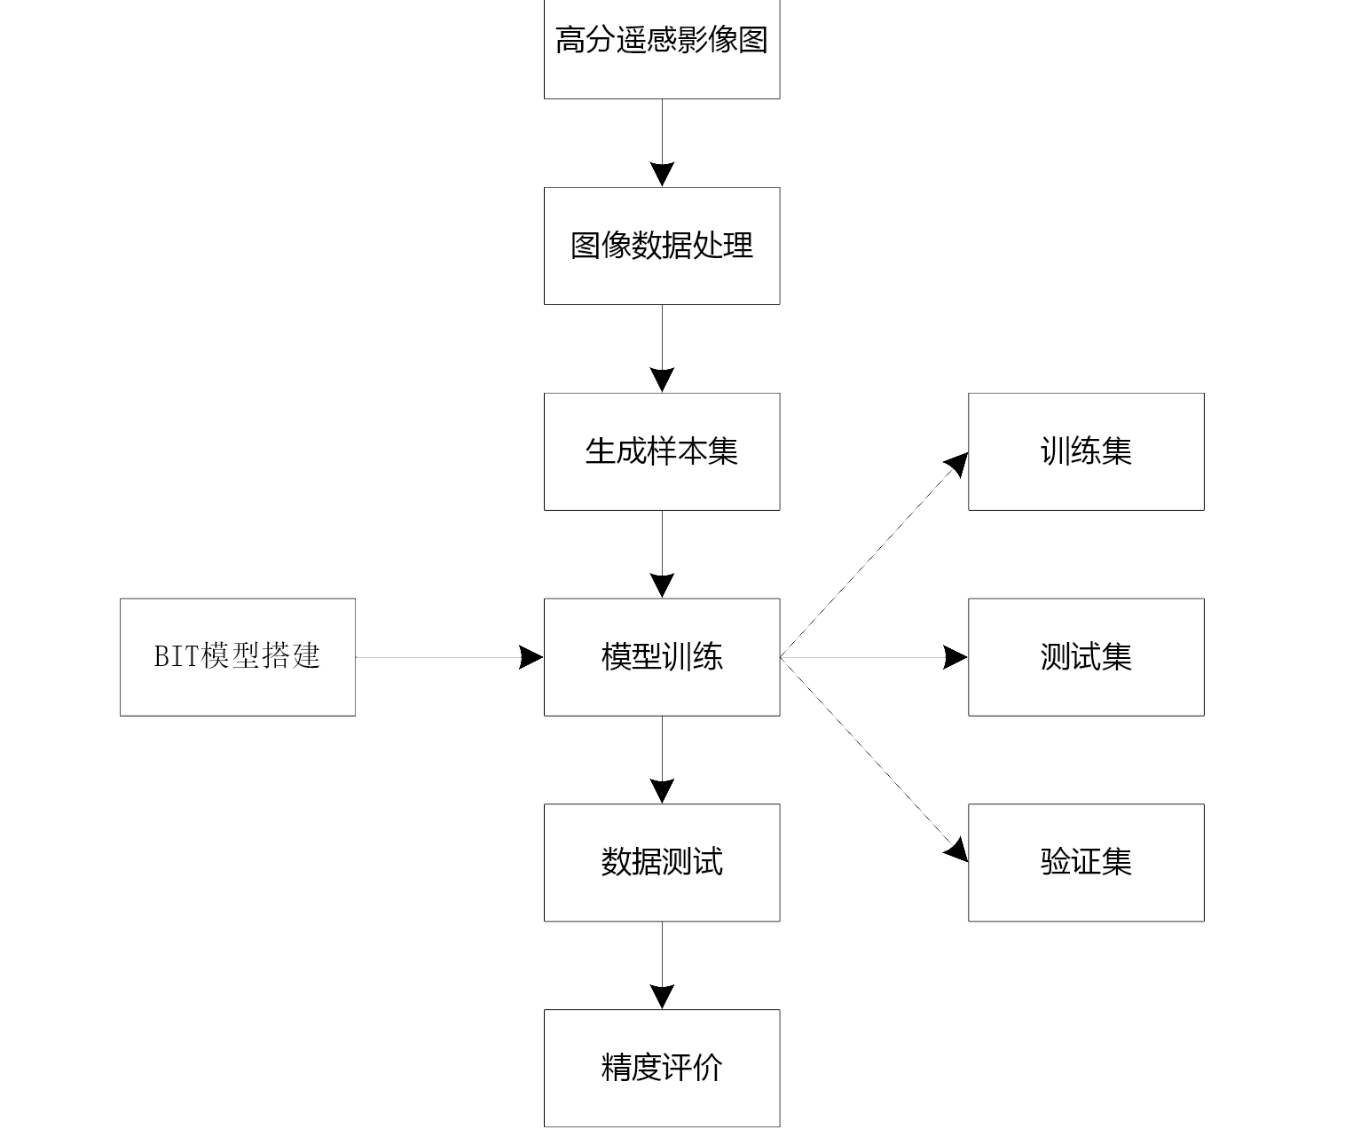
\includegraphics[width=0.8\textwidth]{项目计划书图片/image25.png}
    \caption{简单的技术路线}
    \label{fig:9}
\end{figure}

\subsection{2.部署方式与适配性}

系统采用前后端轻量化架构，普通电脑即可本地化部署运行，无需专业服务器支持；同时兼容GF-2卫星影像与无人机航拍影像，适配多源数据采集场景，可满足大范围卫星批量监测与重点区域无人机现场核查的双重需求。

在架构上，后端基于 FastAPI 承担影像接收、任务调度、模型推理与结果组织，前端可视化 Web 系统提供影像上传、变化检测、结果可视化、AI 解读与一键报告等功能模块，二者通过标准接口解耦，使算法模型迭代不必牵动前端交互逻辑。轻量化带来的直接价值是部署门槛下降：区县一级的农业技术推广或土地管理机构利用现有办公计算机即可搭建运行，无需专用服务器集群；影像与解译成果在本地完成处理与存储，也减少了敏感地理信息的外链流转。在多源适配方面，GF-2亚米级光学影像覆盖范围广、重访周期稳定，适合大范围批量普查；无人机航拍影像分辨率更高、观测角度灵活，适合对疑点图斑开展现场核查，系统以统一规范组织两类影像，使“卫星普查—无人机核查”能在同一平台内闭环完成。

“卫星普查—无人机核查”两级作业模式的配合，关键在于两类数据在统一空间基准与统一处理规范下衔接。卫星端承担面状覆盖，按周对试点区耕地开展全域比对，输出疑点图斑清单，明确其位置、范围与疑似变化类型；无人机端按清单开展点状核查，对交通不便、地块零碎或影像受云影遮挡的区域低空补测，获取分辨率更高的正射影像与局部细节。两级成果在同一平台内叠加显示，核查结论可以直接回填到卫星图斑上，形成“发现—核验—确认”的固定流程，避免两套数据各自成图、结论难以对应。这种分工在成本上同样合理：面状普查交由重访周期稳定的卫星完成，而受空域审批与天气条件制约的低空作业只投放在真正需要的疑点区域。

\subsection{3.一线友好的使用体验}

系统设计充分考虑基层用户需求，无需遥感专业知识，基层农技人员即可独立操作；性能上，系统采用轻量化模型与批量化推理策略，在保证精度的同时实现了高效率处理，大幅降低了一线监测的人力与时间成本。

从使用流程看，基层人员只需完成影像上传，系统即自动完成变化检测计算、结果渲染与报告生成：变化图斑的位置、范围与类别以可视化图层叠加呈现，无需解读复杂的指数图或波段组合；AI 解读模块以自然语言说明图斑的变化性质与可能成因；一键报告功能将检测结论与关键截图整合为规范化成果文档，使遥感解译的专业门槛被转移至系统内部。在性能上，轻量化模型使交互式操作几乎感受不到等待，批量化推理能力则保证在周级监测频次下足以支撑较大范围区域的批量作业，不会因算力不足而被迫降低监测频次或压缩覆盖范围。

\section{十、项目核心知识产权成果}

本项目在技术研发过程中，形成了以软件著作权与实用新型专利为核心的完整知识产权保护体系，为技术方案的原创性、先进性与可落地性提供了坚实支撑，具体成果如下：

\subsection{1.计算机软件著作权（3项）}

团队成员围绕黑土地遥感监测、耕地变化识别、数据处理与智能分析等核心业务模块，共完成3项计算机软件著作权登记，覆盖了从影像预处理、算法运算到成果可视化的全流程软件系统，充分证明项目软件系统的原创性与独立开发能力，为后续平台迭代与推广应用筑牢了法律基础。

\begin{itemize}
    \item 影像预处理模块：完成辐射校正、几何配准与质量筛查，为算法运算提供规范、可比对的双时相数据基础。
    \item 算法运算模块：承载改进 BIT 双时相 Transformer 模型推理，以 ResNet18为 CNN 骨干网络提取特征，通过语义分词器抽取语义 tokens。
    \item 成果可视化模块：提供影像上传、变化检测、结果可视化、AI 解读与一键报告等交互功能，将算法输出转化为业务决策可用的直观成果。
\end{itemize}

三项登记的完成明确了成果的权利归属，也为技术方案的推广复制保留了稳定的权利基础。

团队成员的计算机软件著作权共计3项，上述内容即为其全部登记成果，不存在其他未列明的登记项。三项登记沿“采集—解译—应用”链条依次落位：影像预处理模块把住数据入口的质量关，解决多源影像在辐射与几何上的可比性问题；算法运算模块承载改进 BIT 双时相 Transformer 的核心推理逻辑；成果可视化模块面向最终使用者，把模型输出转化为可理解、可汇报的业务成果。三者首尾相接、彼此支撑，任一环节缺失都会削弱整条数据链的可用性。

\subsection{2.实用新型专利（1项，已授权）}

项目核心技术方案《一种用于图像采集的遥感无人机》已获国家知识产权局实用新型专利授权，专利号 ZL 2025 2 2047856.0，授权公告号 CN 224511490 U，专利申请日为2025年9月24日，授权公告日为2026年7月17日，专利权人为黑龙江八一农垦大学。该专利聚焦于遥感数据采集与处理的关键创新点，进一步强化了项目在算法与技术实现层面的核心竞争力，为技术成果转化与市场应用构建了知识产权壁垒。

该专利针对的是数据链条最前端的采集环节：在“天空地一体化”体系中，无人机承担高分辨率、高灵活性地获取重点区域影像的职责，其采集质量直接决定后续解译成果的上限。将关键采集方案纳入专利布局，使项目实现了对“采集—解译—应用”全链条中数据入口环节的知识产权覆盖，与算法层面的软件著作权互补，构成从硬件采集方法到软件解译系统的立体保护。

软件著作权与实用新型专利的组合，使保护范围覆盖了从硬件采集方法到软件解译系统的完整链条：专利锁定数据入口环节，保护采集装置与作业方法层面的原创贡献；软件著作权锁定数据处理与成果输出环节，保护代码实现与系统功能层面的原创表达。二者在权利类型上互补，即便他人在硬件上采用不同实现路径，只要复用了本系统的解译与可视化功能，仍会落入软件著作权的保护范围。这种立体布局为后续技术成果转化、平台推广与对外合作划定了可界定的权利边界。

\begin{figure}[htbp]
    \centering
    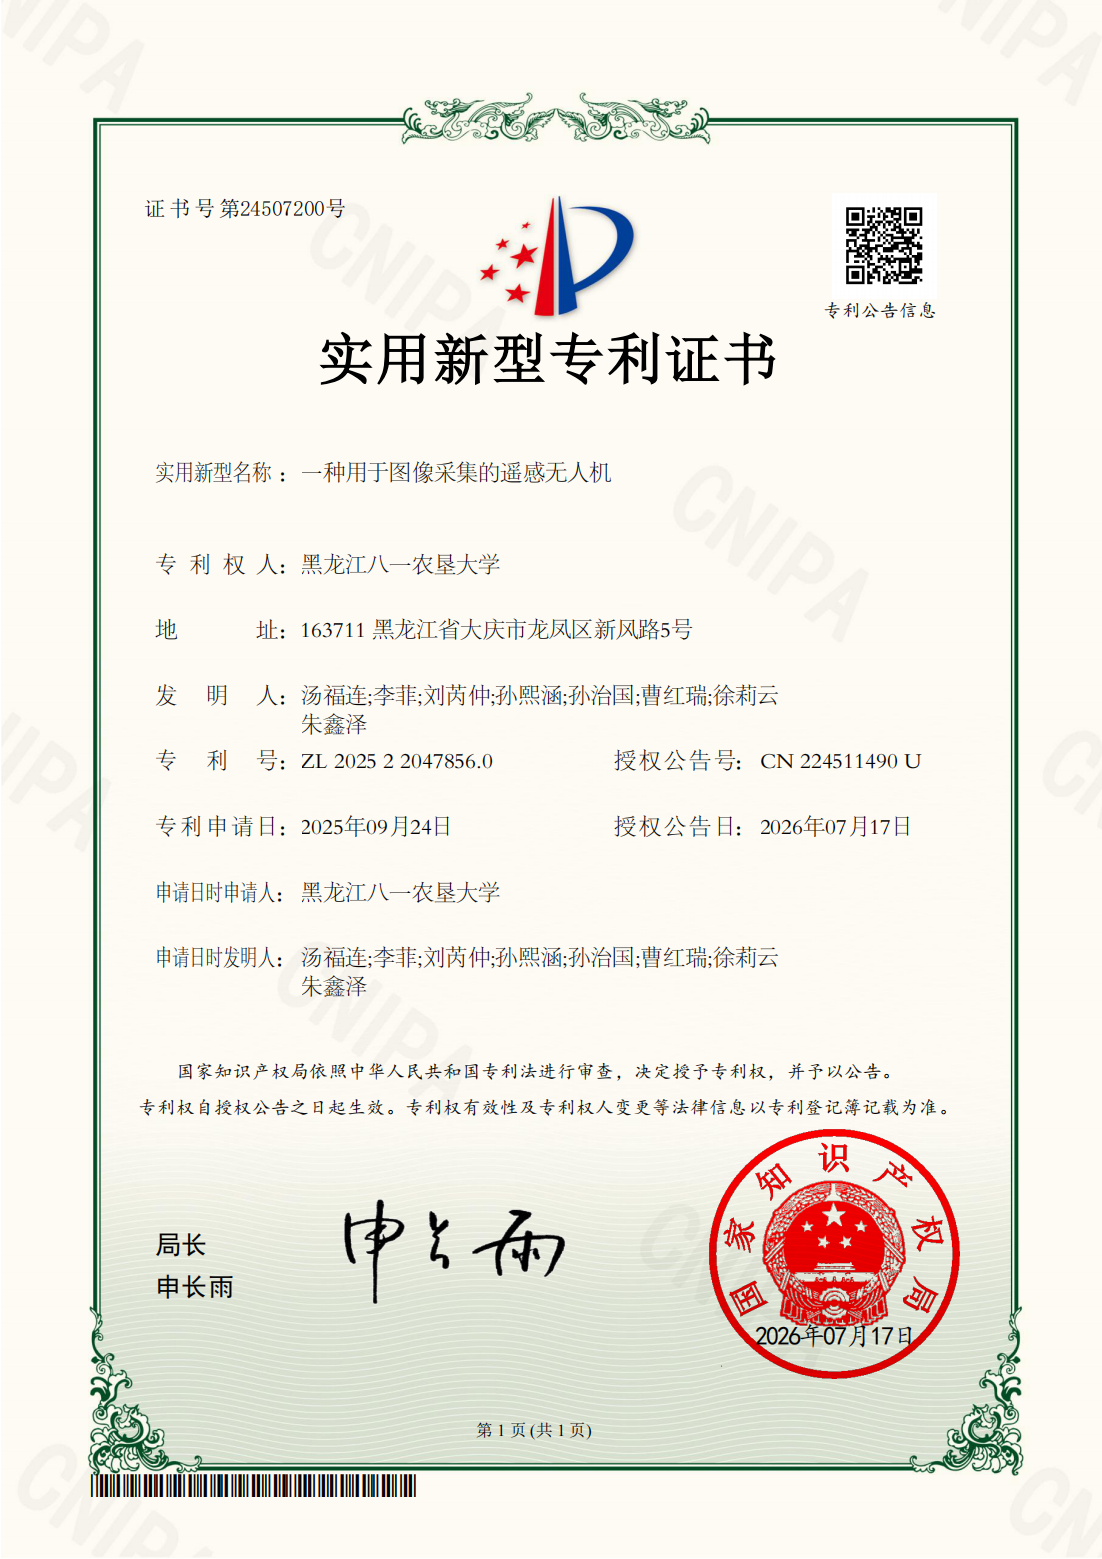
\includegraphics[width=0.8\textwidth]{项目计划书图片/image26.png}
    \caption{实用新型专利证书（专利号 ZL 2025 2 2047856.0）}
    \label{fig:10}
\end{figure}

\begin{figure}[htbp]
    \centering
    
\includegraphics[width=0.8\textwidth]{项目计划书图片/image27.png}
    \caption{计算机软件著作权登记证书（一）}
    \label{fig:11}
\end{figure}

\begin{figure}[htbp]
    \centering
    
\includegraphics[width=0.8\textwidth]{项目计划书图片/image28.png}
    \caption{计算机软件著作权登记证书（二）}
    \label{fig:12}
\end{figure}

% ==================== 片段 g8 ====================
\section{十一、项目模式}

本项目在技术路径与推广路径上分别形成了可复制的运作模式，二者共同构成从技术研发到基层服务的完整闭环。

\subsection{（1）技术研发模式：数据+模型双轮驱动}

\subsubsection{（1）以精准识别为核心，打造适配黑土场景的专属技术底座}

通用遥感变化检测模型多基于城市地表、道路、建筑等语义类别构建样本，其光谱与纹理统计特征与东北黑土区连片耕地差异显著：黑土耕地地表覆盖均质度高、作物物候引起的时相差异明显、地块边界依赖田埂与垄沟等弱特征，直接迁移通用模型易出现漏检与误检。为此，项目确立“数据先行、模型跟进、二者交替迭代”的研发思路，将数据建设与算法优化同步推进。

\textbf{数据支撑}：项目自建黑土影像数据集，针对东北黑土地域的光谱、纹理特征构建专属样本库，系统标注耕地撂荒、非农占用、侵蚀沟等典型变化类型，解决通用数据集对黑土区耕地变化识别不准的问题。样本库兼顾不同季节、不同作物与不同地形条件，使模型在真实业务场景中具备稳定的泛化能力；新采集的影像与基层核查反馈的变化图斑可回补入库，为模型持续迭代提供数据源头。

\textbf{算法优化}：项目采用改进的 BIT（Bipartite Transformer）双时相 Transformer 模型，以 ResNet18作为 CNN 骨干网络提取双时相影像的多尺度空间特征，并通过核心子模块“语义分词器”将特征图切分为语义 tokens，在前后两个时相之间建立长距离的语义关联，从而通过对比不同时期的卫星影像，精准捕捉耕地撂荒、非农占用等变化。该结构对地块内部的一致性与地块之间的边界变化均有较好响应，对细小、狭长的变化区域尤为敏感。在此基础上，项目持续迭代优化模型参数，在保证识别精确率达到既定指标的前提下，不断提升检测精度与效率，使模型在精度与算力开销之间取得更优平衡。

数据与模型的交替迭代构成研发模式的运转机制：新采集的影像经人工与算法协同标注进入样本库用于再训练，更新后的模型回流业务场景生成新的变化图斑，图斑经基层核查后再次回补入库。这一循环使精度提升不依赖一次性的大规模标注投入，而随监测范围扩大持续累积。项目选择轻量化骨干网络配合语义分词的组合，在识别精确率达标的前提下压缩算力开销，使模型兼顾专业核查与基层部署两类场景。

\subsection{（2）落地服务模式：平台+基层打通最后一公里}

技术成果只有进入基层工作流程才能转化为保护效益；现实中遥感监测成果往往停留在专业软件与专题图件中，形成“有发现、无响应”的断层。项目以轻量化、易使用为目标，从工具与流程两端降低使用门槛。

\textbf{（1）轻量化部署}：项目采用前后端分离架构，后端基于 FastAPI 构建服务接口，前端为可视化 Web 系统，功能覆盖影像上传、变化检测、结果可视化、AI 解读与一键报告生成，形成完整的业务操作链路。系统降低平台运行门槛，普通电脑即可流畅使用，无需专业设备支撑，适配乡镇、合作社等基层场景，使基层工作人员无需掌握遥感专业软件即可完成日常监测任务；一键报告功能将检测结果自动整理为规范文档，减少人工汇总与制表的重复劳动。

\textbf{（2）闭环预警服务}：项目向农户、合作社直接推送耕地撂荒、违规占用等预警信息，打破“监测—响应”的信息壁垒，打通耕地保护的“最后一公里”。预警信息并非孤立推送，而是与变化图斑的位置、面积、类型及处置建议一并送达，使基层主体能够直接开展核查与处置，形成发现、核实、反馈的完整链条，将原本分散的“监测”与“响应”连接为可追溯的责任链。

从运作流程看，落地服务模式由“监测—推送—核查—反馈”四个环节构成：系统按周更新影像并完成变化检测，将疑似变化图斑按行政区划与经营主体归集，推送至乡镇、合作社与农户；基层主体收到信息后开展实地核查，核查结论回填系统并作为后续监测与样本更新的依据。为保障服务可持续，项目以培训本地人员、扶持本地化服务团队的方式承接日常运维，使服务能力沉淀在基层，避免项目结束、服务中断。

\subsection{（3）项目核心支撑亮点}

两大模式的落地，依托七大核心特点形成完整支撑体系：

\begin{enumerate}
  \item \textbf{数据驱动}：以黑土专属影像数据为基础，为模型迭代和监测精度提供持续保障。
  \item \textbf{轻量部署}：算法与平台轻量化改造，降低基层使用门槛，实现“开箱即用”。
  \item \textbf{周级监测}：以周为周期更新影像数据，实现耕地变化的高频动态监测。
  \item \textbf{基层适配}：功能设计贴合乡镇、村集体的实际工作场景，操作简单易上手。
  \item \textbf{预警闭环}：从异常识别到信息推送，形成完整的监测预警与响应闭环。
  \item \textbf{国产遥感}：依托国产卫星影像数据，保障数据安全与自主可控。项目以国产高分二号（GF-2）亚米级光学遥感卫星影像为主要数据源，并辅以无人机航拍影像作为机动补充，在数据获取环节即实现自主可控。
  \item \textbf{用养结合}：将监测预警与耕地养护、政策服务相结合，实现“监测即服务”，助力黑土资源可持续保护。
\end{enumerate}

七大亮点构成层层递进的支撑逻辑：数据驱动与国产遥感回答“数据从哪里来”，轻量部署与基层适配回答“谁来用、是否用得起”，周级监测与预警闭环回答“发现之后怎么办”，用养结合回答“监测的最终目的”。

进一步看，七个亮点是按“数据基础—使用门槛—响应机制—最终目标”四个层次组织的：数据驱动与国产遥感位于底层，决定监测能力能否自主稳定供给；轻量部署与基层适配位于工具层，决定技术能否被一线人员真正掌握；周级监测与预警闭环位于机制层，决定发现的问题能否转化为实际处置；用养结合位于目标层，决定监测的落点是否回到黑土地质量本身。任一层次缺失，其他层次的成效都会被削弱。

\subsection{（4）保险定损服务模式：明确付费方}

前述研发模式与落地服务模式回答了“怎么做”与“给谁用”，但尚未回答“谁付费”。项目在试点中形成的判断是：面向农户与合作社的预警服务应当保持免费，其成本由监测服务的另一类使用者承担，即农业保险机构。

这一判断来自定损环节的现实成本结构。按行业公开报道的数据，传统人工实地查勘的作业成本约为每亩 8 至 12 元，而基于遥感的变化检测与定损可将单位面积成本降至每亩 2 至 5 元；在作业周期上，人工查勘受限于人力调度与地块分散，理赔周期通常以周计，遥感辅助定损可将周期压缩至数日。对于承保面积动辄数十万亩的保险机构而言，这一差异直接体现为可观的成本节约与赔付时效提升。

项目据此形成的服务模式是：面向农户与合作社的耕地变化预警保持免费推送，作为数据回传与样本积累的入口；面向保险机构的灾情范围核定与损失估算则作为有偿服务提供，收入用于覆盖平台运维与样本标注成本。两类使用者共享同一套检测能力，而付费主体与免费主体明确分离，使服务在农户侧不设门槛的同时具备自我维持的可能。

需要如实说明的是，上述单位面积成本与周期数据来自行业公开报道，并非本项目在试点区域的实测结果；保险机构对定损结果的实际采纳程度，还取决于其结果能否通过抽样实测校验这一前提。项目当前的工作重心，正是通过试点区域的地面核查数据持续标定模型置信度与真实减产之间的换算关系，为定损结果进入理赔流程提供依据。

\section{十二、项目核心收益：黑土智能检测系统}

本项目自研的黑土智能检测系统，通过 BIT 模型与轻量化部署技术，实现了黑土地变化监测的效率、成本与精度的三重突破，核心成果与收益如下：

\subsection{1.核心性能指标}

\begin{itemize}
  \item \textbf{识别精度}：BIT 模型对黑土地变化类别的识别精确率达70\%，可有效识别耕地撂荒、非农占用、侵蚀沟等关键变化类型，满足黑土地精细化监测的需求。该指标面向黑土区真实业务场景下的多类别变化识别任务，其意义在于系统输出的变化图斑中相当一部分可直接用于基层核查，从整体上降低人工复核工作量。
  \item \textbf{成本优化}：相较传统深度学习方案，算力成本降低约69\%，大幅降低了监测系统的部署与运行门槛。成本下降主要来自骨干网络的轻量化设计与前后端分离的轻量架构：前者减少单次推理的算力开销，后者使系统无需依赖高端硬件即可运行，从而把监测能力从专业机房延伸到基层办公环境。
  \item \textbf{效率提升}：从传统人工/常规遥感方法到本系统，单次监测周期缩短约33\%，实现了黑土地变化的高频动态监测。其价值不仅在于时间本身，更在于使“周级”更新成为常态化能力：监测频次提高意味着变化能够被更早发现，处置窗口相应前移，使耕地保护由事后统计转向事中干预。
\end{itemize}

三项指标并非彼此孤立，而是共同决定系统能否在真实业务中成立：识别精确率决定输出结果能否作为核查依据，算力成本决定系统能否下沉到基层办公环境，监测周期决定变化能否在处置窗口内被发现。三者结合，意味着系统在“看得准、用得起、发现得早”三方面同时具备可用性。

\subsection{2.验证与落地基础}

系统已在松嫩平原完成实地验证，适配普通电脑即可部署运行，无需高端硬件支撑，为后续在东北黑土区的规模化推广奠定了坚实基础。松嫩平原黑土分布集中、耕地经营主体类型丰富，其验证结论对东北其他黑土区具有较强的参考意义与可迁移性。

\subsection{3.业务与社会价值}

系统直接服务于黑土地保护“总量不减少、功能不退化”的核心目标，为黑土地常态化监测、耕地保护政策落地提供了智能化支撑，助力实现黑土地退化问题的“早发现、早预警、早治理”，兼具显著的生态效益与社会效益。

在业务层面，系统将《中华人民共和国黑土地保护法》《国家黑土地保护工程实施方案（2021—2025年）》《东北黑土地保护性耕作行动计划（2020—2025年）》等政策文件提出的监测与保护要求，转化为可操作、可查询、可追溯的信息化工具，使政策要求与基层执行之间有了明确的技术衔接点。在社会层面，系统面向农户与合作社免费提供预警服务，降低了小规模经营主体获取专业监测信息的门槛，使黑土地保护由少数专业机构的职责扩展为多方共同参与的日常实践。

\section{十三、项目成效与发展规划}

\subsection{1.当前项目成效}

赋能基层，带动多方价值。项目落地以来，已在农业帮扶与带动就业两方面取得了显著成效：

\begin{enumerate}
  \item \textbf{农业帮扶}：免费为农户推送撂荒、违法占用预警，已帮助500+农户提前止损；同时为10万亩黑土地提供“监测—诊断—措施”的全链条服务，助力黑土地用养结合，提升耕地质量。所谓“提前止损”，是指农户在违规行为造成不可逆后果之前即获得提示，有机会及时恢复耕种或纠正用地行为；全链条服务则使监测结果不止于发现问题，还能对接养护建议与政策服务。
  \item \textbf{带动就业}：通过培训基层农技员与返乡青年，新增智能监测岗位30+个；推广轻量化设备操作，扶持大学生创业与本地化服务团队；建立黑土地影像标注协作点，带动当地农户家门口就业，实现技术赋能与乡村振兴的结合。受训的基层人员既服务于本项目，也逐步成为当地黑土地保护工作的长期技术力量。
\end{enumerate}

农业帮扶与带动就业互为支撑：帮扶扩大监测服务覆盖面，岗位增设保障服务持续下沉到田间地头。

从可持续性看，两项成效共同指向“输血”与“造血”的结合：免费预警服务直接降低农户的损失风险，属于短期可感知的帮扶；岗位增设、设备操作培训与影像标注协作点则把监测工作拆解为基层可承接的环节，使农户与返乡青年在参与中获得技能与收入来源。影像标注协作点尤其关键，它既是模型迭代所需样本的生产端，也是本地就业的容纳端。

\subsection{2.项目发展历程与未来规划}

项目从2022年启动至今，已完成从调研到试点的关键阶段，并规划了清晰的长期发展路径：

\begin{table}[htbp]
  \centering
  \caption{项目发展历程与未来规划}
  \begin{tabular}{|c|p{0.68\textwidth}|}
  \hline
  时间节点 & 阶段目标与主要任务 \\
  \hline
  2022年 & 启动政策调研与数据积累，完成黑土地现状摸底 \\
  \hline
  2024年 & 完成影像标注与模型验证，实现技术闭环 \\
  \hline
  2026年 & 获得软件著作权并落地试点，形成成熟的产品形态 \\
  \hline
  2028年 & 推广至黑、吉、辽、蒙四省区，实现常态化监测 \\
  \hline
  2030年 & 构建“天空地”一体化监测网，实现东北黑土地全网动态监测 \\
  \hline
  \end{tabular}
  \label{tab:plan}
\end{table}

五个时间节点层层递进：2022年解决“有无依据与数据”，2024年解决“技术是否成立”，2026年解决“成果能否落地”，2028年解决“能否跨区域复制”，2030年则指向“能否形成全域覆盖的一体化监测能力”，前一阶段的产出构成后一阶段的输入。

具体来看，2022年的调研与数据积累为后续工作确立了地域范围与问题清单；2024年的影像标注与模型验证解决了技术是否成立的问题，使研发转为可复现的成果；2026年团队获软件著作权3项并落地试点，标志成果具备可交付的产品形态；2028年推广至黑、吉、辽、蒙四省区，重点在于把验证过的方案复制到气候、地形与经营方式不同的区域；2030年构建“天空地”一体化监测网，形成覆盖东北黑土区的常态化监测能力。

展望未来，项目将继续以双轮驱动夯实技术底座、以平台与基层贯通拓展应用边界，围绕黑土地保护“总量不减少、功能不退化”的核心目标持续发力，为东北黑土区的耕地保护提供长期、稳定、自主可控的技术支撑。

% ==================== 片段 team ====================
\section{十四、团队介绍与分工}

\subsection{1.团队构成与分工}

本项目由 4 名成员组成，覆盖算法、后端、前端与数据处理等方向，形成分工明确、协同高效的研发团队：由项目负责人统筹全局并主导核心技术攻关，后端成员承担服务端开发与测试，前端与数据成员负责界面实现与数据集构建。

\begin{table}[htbp]
\centering
\caption{团队成员分工与贡献}
\begin{tabular}{|p{1.9cm}|p{2.6cm}|p{6.6cm}|p{3.0cm}|}
\hline
\textbf{姓名} & \textbf{角色} & \textbf{主要工作} & \textbf{贡献说明} \\
\hline
汤福连 & 项目负责人 & 全局统筹；系统架构设计；模型训练（BIT，ResNet18 骨干）；后端 API 核心开发；前端总体设计；AI 与 GIS 集成；测试与安全加固；云服务器部署上线 & 项目核心，独立完成模型、后端、前端主体与部署上线的绝大部分工作 \\
\hline
刘芮仲 & 后端开发 & 后端部分接口开发；测试用例编写；文档与资料整理 & 参与后端开发与测试，辅助主干工作 \\
\hline
张珏枫 & 后端开发 & 后端辅助接口开发；数据库与部署运维协助；问题排查 & 参与后端辅助与部署协作 \\
\hline
于欣欣 & 前端与数据标注 & 前端页面辅助开发；高德地图 API 集成；自建黑土耕地数据集像素级标注 & 参与前端与数据标注工作 \\
\hline
\end{tabular}
\end{table}

从分工结构看，团队以“算法—后端—前端—数据”为主线组织协作：算法与架构由项目负责人统一把关，保证技术路线的一致性；后端成员在统一接口规范下并行开发，避免相互阻塞；前端与数据成员则分别对接系统界面与数据集构建，形成从数据到应用的完整链条。这一结构在项目周期紧、任务跨度大的条件下，有效保证了研发进度与成果质量。

\subsection{2.协作机制}

团队在研发过程中建立了规范、可追溯的协作机制，具体包括：

\begin{itemize}
    \item \textbf{版本管理}：全程使用 Git 进行代码管理，提交采用语义化格式（feat/fix/chore），关键版本打标签，全部变更可回溯、可审计。
    \item \textbf{接口先行}：前后端以 OpenAPI 接口文档为契约并行开发，前端按接口约定独立推进，降低联调耦合与等待成本。
    \item \textbf{数据双人复核}：自建黑土耕地数据集采用“独立标注 + 交叉验证”流程，由两名成员分别标注并交叉核对，降低标注噪声对模型精度的影响。
    \item \textbf{环境统一}：开发、测试与生产环境通过容器化与统一配置模板保持一致，避免“本地可运行、上线即报错”的常见问题。
    \item \textbf{工具提效}：研发过程中引入 AI 编码辅助工具参与需求梳理、代码审查与安全加固，提升迭代效率与代码质量。
\end{itemize}

上述机制使团队在有限人力条件下完成了从模型训练、系统开发到安全加固、部署上线的全流程工作，也为成果的后续维护与推广保留了良好的工程基础。

% ==================== 片段 refs ====================
\renewcommand{\refname}{十五、参考文献}

\begin{thebibliography}{99}

\bibitem{ref1} Hao Chen, Zipeng Qi, Zhenwei Shi. Remote Sensing Image Change Detection with Transformers[J]. IEEE Transactions on Geoscience and Remote Sensing, 2021.

\bibitem{ref2} 余银峰, 贾振红, 覃锡忠, 杨杰, 庞韶宁. 遥感图像变化检测算法研究[J]. 计算机工程与应用, 2011(25).

\bibitem{ref3} 蒋世豪, 江洪. 基于 GDAL 的遥感图像变化检测技术[J]. 计算机工程与应用, 2020(16).

\bibitem{ref4} Tianyu Yan, Zifu Wan, Pingping Zhang. Fully Transformer Network for Change Detection of Remote Sensing Images[J].

\bibitem{ref5} Xinyang Song, Zhen Hua, Jinjiang Li. Remote Sensing Image Change Detection Transformer Network Based on Dual-Feature Mixed Attention[J]. IEEE Transactions on Geoscience and Remote Sensing, 2022.

\bibitem{ref6} 宋小丽, 李炜明. 基于图像匹配的遥感图像建筑物变化检测[J]. 微计算机信息, 2008(19).

\bibitem{ref7} M. Zhang, G. Xu, K. Chen, M. Yan, X. Sun. Triplet-based Semantic Relation Learning for Aerial Remote Sensing Image Change Detection[J]. IEEE Geoscience and Remote Sensing Letters, 2019, 16(2): 266--270.

\bibitem{ref8} Jingming Li, Panpan Zheng, Liejun Wang. Remote Sensing Image Change Detection Based on Lightweight Transformer and Multiscale Feature Fusion[J]. IEEE Journal of Selected Topics in Applied Earth Observations and Remote Sensing, 2025.

\bibitem{ref9} ``\ldots networks,'' Remote Sensing, vol. 12, no. 6, p. 901, 2020.
% 注：原文此条与上一条粘连、作者与标题信息缺失，作者可自行补全。

\end{thebibliography}

% ==================== 片段 appendix ====================
\setcounter{table}{0}
\renewcommand{\thetable}{A-\arabic{table}}

\section{附录 A　高分二号（GF-2）卫星技术参数}

本附录汇总高分二号（GF-2）卫星的公开技术参数，作为正文第七章“项目技术的支撑”的资料性补充。正文侧重说明各参数与本项目监测需求的对应关系，本附录则给出完整的技术清单，便于查阅与核对。表中参数依据该卫星官方公布数据整理。

\subsection{A.1 平台与载荷主要参数}

\begin{table}[htbp]
    \centering
    \caption{高分二号（GF-2）卫星平台与载荷主要参数}
    \label{tab:gf2-platform}
    \small
    \begin{tabular}{|p{3.4cm}|p{5.4cm}|p{4.6cm}|}
        \hline
        \textbf{参数项} & \textbf{技术指标} & \textbf{说明} \\
        \hline
        发射时间 & 2014 年 8 月 19 日 & 于太原卫星发射中心发射 \\
        \hline
        轨道类型 & 太阳同步回归轨道 & 降交点地方时约上午 10:30 \\
        \hline
        轨道高度 & 631 km & 兼顾覆盖范围与成像分辨率 \\
        \hline
        回归周期 & 69 天 & 不侧摆成像时的全球覆盖周期 \\
        \hline
        侧摆能力 & $\pm35^{\circ}$ & 具备快速姿态机动能力 \\
        \hline
        重访周期 & 侧摆条件下约 5 天 & 满足“周级”动态监测的频次需求 \\
        \hline
        全色分辨率 & 星下点 0.8 m & 我国首颗分辨率优于 1 m 的民用光学遥感卫星 \\
        \hline
        多光谱分辨率 & 星下点 3.2 m & 与全色影像融合后提升地类判别能力 \\
        \hline
        成像幅宽 & 45 km & 由两台相机拼接实现 \\
        \hline
        定位精度 & 无地面控制点时约 50 m（CE90） & 保障多时相影像的几何配准精度 \\
        \hline
    \end{tabular}
    \par\vspace{2pt}
    {\footnotesize 注：表中“星下点”指卫星垂直投影点处的成像分辨率，为载荷实际成像指标；相机标称指标为全色 1 m、多光谱 4 m。}
\end{table}

\subsection{A.2 谱段设置与主要用途}

\begin{table}[htbp]
    \centering
    \caption{高分二号（GF-2）卫星谱段设置及本项目用途}
    \label{tab:gf2-bands}
    \small
    \begin{tabular}{|p{2.4cm}|p{3.4cm}|p{7.6cm}|}
        \hline
        \textbf{谱段} & \textbf{波长范围} & \textbf{主要用途} \\
        \hline
        全色 & 0.45--0.90 $\mu$m & 提供高分辨率灰度影像，用于地块边界、田埂与侵蚀沟等几何细节判读 \\
        \hline
        蓝 & 0.45--0.52 $\mu$m & 水体识别与大气校正，辅助地表反射率反演 \\
        \hline
        绿 & 0.52--0.59 $\mu$m & 表征植被反射特征，用于作物长势与植被覆盖监测 \\
        \hline
        红 & 0.63--0.69 $\mu$m & 叶绿素吸收波段，与近红外组合可计算 NDVI 等植被指数 \\
        \hline
        近红外 & 0.77--0.89 $\mu$m & 对植被与土壤水分敏感，用于植被覆盖度与土壤有机质反演 \\
        \hline
    \end{tabular}
\end{table}

\subsection{A.3 本项目的数据使用方式}

在本项目中，上述影像按以下方式进入业务流程：首先对全色与多光谱影像进行辐射定标与大气校正，并以全色影像为基准完成几何配准，使两个时相的影像在同一空间基准上逐像元对应；随后进行全色与多光谱融合，在保留多光谱信息的同时将空间分辨率提升至全色水平；最后将融合影像统一裁剪为 $256 \times 256$ 像素的影像块，作为变化检测模型的输入。

四类多光谱谱段在其中承担不同职责：可见光波段（蓝、绿、红）用于地类判别与植被指数计算，近红外波段则提供植被与土壤水分信息，二者结合使模型不仅能判断“地表是否发生变化”，还能为变化类型的判别提供光谱依据。这一处理流程与正文所述的“数据采集—智能检测—分析决策”技术闭环相衔接，是其中数据环节的具体实现方式。

% ==================== 片段 appendix_b ====================
\setcounter{table}{0}
\renewcommand{\thetable}{B-\arabic{table}}

\section{附录 B　项目成果数据汇总}

本附录汇总项目在检测精度、运行效率、应用成效、系统规模与知识产权等方面形成的成果数据。其中性能与应用成效数据口径与正文一致；模型训练指标取自项目训练日志的实测记录，可逐轮复核。

\subsection{B.1 核心性能指标}

\begin{table}[htbp]
    \centering
    \caption{项目核心性能指标}
    \label{tab:perf}
    \small
    \begin{tabular}{|p{2.6cm}|p{4.4cm}|p{3.6cm}|p{3.2cm}|}
        \hline
        \textbf{指标类别} & \textbf{指标} & \textbf{指标值} & \textbf{说明} \\
        \hline
        检测精度 & 黑土地变化识别精确率 & 70\% & 试点应用验证结果 \\
        \hline
        运行成本 & 算力成本 & 较传统深度学习方案降低 69\% & 相较同类高算力方案 \\
        \hline
        监测时效 & 单次监测任务周期 & 较人工/常规遥感方法缩短 33\% & 指单次作业周期（不含影像重访等待时间）；成果更新频次为周级 \\
        \hline
    \end{tabular}
    \par\vspace{2pt}
    {\footnotesize 注：检测精度指黑土地变化类别的识别精确率，与模型训练过程中在公开基准数据集上测得的 mF1 指标口径不同，二者不应直接比较（见 B.4）。}
\end{table}

\subsection{B.2 应用成效}

\begin{table}[htbp]
    \centering
    \caption{项目应用成效}
    \label{tab:effect}
    \small
    \begin{tabular}{|p{3.0cm}|p{4.4cm}|p{3.0cm}|p{3.4cm}|}
        \hline
        \textbf{成效类别} & \textbf{指标} & \textbf{数值} & \textbf{说明} \\
        \hline
        农业帮扶 & 服务农户 & 500+ 户 & 免费推送撂荒与违法占用预警 \\
        \hline
        农业帮扶 & 覆盖耕地面积 & 10 万亩 & 提供“监测—诊断—措施”全链条服务 \\
        \hline
        带动就业 & 新增智能监测岗位 & 30+ 个 & 培训基层农技员与返乡青年 \\
        \hline
    \end{tabular}
\end{table}

\subsection{B.3 系统规模}

\begin{table}[htbp]
    \centering
    \caption{系统建设规模}
    \label{tab:scale}
    \small
    \begin{tabular}{|p{5.4cm}|p{2.6cm}|p{6.4cm}|}
        \hline
        \textbf{项目} & \textbf{数量} & \textbf{说明} \\
        \hline
        集成变化检测模型 & 7 种 & 含 BIT、SNUNET、CHANGEFORMER、AFCF3D 等 \\
        \hline
        后端 API 端点 & 40+ 个 & 覆盖认证、检测、AI、历史、地块等模块 \\
        \hline
        前端功能页面 & 16 个 & 单页应用，支持中英双语与深浅主题 \\
        \hline
        系统测试用例 & 54 项 & 通过 53 项，通过率 98.1\% \\
        \hline
    \end{tabular}
\end{table}

\subsection{B.4 模型训练指标（实测记录）}

\begin{table}[htbp]
    \centering
    \caption{变化检测模型训练配置与实测指标}
    \label{tab:train}
    \small
    \begin{tabular}{|p{3.4cm}|p{4.6cm}|p{2.4cm}|p{4.0cm}|}
        \hline
        \textbf{项目} & \textbf{配置/指标} & \textbf{数值} & \textbf{说明} \\
        \hline
        训练数据集 & SYSU-CD 公开基准数据集 & — & 用于模型结构验证 \\
        \hline
        模型结构 & 改进 BIT 双时相 Transformer & — & ResNet18 为 CNN 骨干 \\
        \hline
        输入尺寸 / 批次 & $256 \times 256$ / 4 & — & 二分类（变化/不变） \\
        \hline
        优化器 / 学习率 & SGD / 0.001（线性衰减） & — & 交叉熵损失，100 轮 \\
        \hline
        训练集 mF1 & 首轮 0.699 $\rightarrow$ 末轮 0.907 & — & 逐轮上升，收敛平稳 \\
        \hline
        验证集最佳 mF1 & \textbf{0.8868} & 第 97 轮 & 最佳权重予以固化 \\
        \hline
        末轮验证集指标 & mF1 0.881 / Acc 0.924 / mIoU 0.795 & — & 第 100 轮 \\
        \hline
    \end{tabular}
    \par\vspace{2pt}
    {\footnotesize 注：表中指标为模型在公开基准数据集上的实测结果，取自项目训练日志；正文所述“识别精确率 70\%”为黑土地试点场景下的业务口径指标，两者评价对象与数据来源不同。}
\end{table}

\subsection{B.5 知识产权成果}

\begin{table}[htbp]
    \centering
    \caption{项目知识产权成果}
    \label{tab:ip}
    \small
    \begin{tabular}{|p{3.4cm}|p{2.0cm}|p{3.0cm}|p{6.0cm}|}
        \hline
        \textbf{成果类型} & \textbf{数量} & \textbf{状态} & \textbf{说明} \\
        \hline
        计算机软件著作权 & 3 项 & 已登记 & 覆盖影像预处理、算法运算与成果可视化全流程 \\
        \hline
        实用新型专利 & 1 项 & 已授权 & 《一种用于图像采集的遥感无人机》；专利号 ZL 2025 2 2047856.0，2026 年 7 月 17 日授权公告 \\
        \hline
    \end{tabular}
\end{table}

% ==================== 片段 appendix_c ====================
\setcounter{table}{0}
\renewcommand{\thetable}{C-\arabic{table}}

\section{附录 C　数据集构成与标注规范}

本附录说明项目所用数据集的组成、组织方式与标注规范，作为正文第八章“2.数据支撑”的补充。

\subsection{C.1 数据集组成}

\begin{table}[htbp]
    \centering
    \caption{项目所用数据集的组成与作用}
    \label{tab:ds-compose}
    \small
    \begin{tabular}{|p{3.2cm}|p{2.2cm}|p{3.8cm}|p{5.2cm}|}
        \hline
        \textbf{数据集} & \textbf{类型} & \textbf{影像来源} & \textbf{在本项目中的作用} \\
        \hline
        自建黑土耕地数据集 & 场景数据集 & 高分二号卫星影像、无人机航拍影像 & 面向黑土地场景的模型训练与效果验证，并作为试点应用与系统演示的数据基础 \\
        \hline
        公开基准数据集 & 验证数据集 & 公开遥感影像数据 & 用于模型结构验证与参数调优，使检测方法与同类研究保持可比口径 \\
        \hline
    \end{tabular}
    \par\vspace{2pt}
    {\footnotesize 注：两类数据集在本项目中分工不同——公开基准数据集用于验证模型结构本身是否有效，自建场景数据集用于验证模型在黑土地场景下是否可用。附录 B.4 所列 mF1 指标即在公开基准数据集上测得。}
\end{table}

\subsection{C.2 数据组织方式}

项目影像与标签按四类目录组织，分别存放 A 时相影像、B 时相影像、变化标签与样本清单。每条样本由一对双时相影像与一幅像素级标签构成：两幅影像为同一区域不同时期的观测结果，标签则逐像素标注该区域在该时间段内是否发生变化，变化区域标记为白色、未变化区域标记为黑色。影像在进入模型前统一裁剪为 $256 \times 256$ 像素，以保证输入尺寸一致。

\subsection{C.3 标注规范}

数据标注遵循“采集—配准—标注—核验”的流程，各环节要点如下：

\begin{itemize}
    \item \textbf{影像筛选}：选取时间基线一致、云覆盖较少、成像质量合格的影像对，避免因云影、时相差异过大引入伪变化；
    \item \textbf{几何配准与辐射归一化}：使两个时相的影像在同一空间基准上逐像元对应，并压缩成像条件差异造成的色调偏差；
    \item \textbf{像素级标注}：使用 ArcGIS 等专业工具逐像素勾绘变化区域边界，形成与影像对一一对应的真值标签；
    \item \textbf{交叉复核}：采用双人独立标注并交叉核对的方式控制标注误差，对边界模糊、地类易混淆的样本进行复判或剔除；
    \item \textbf{负样本纳入}：将正常农事活动引起的地表变化（翻耕、收割等）作为负样本纳入数据集，使模型学习“发生了变化但并非退化”的判别边界，降低误判率。
\end{itemize}

上述规范的目的在于保证真值标签的可靠性。变化检测模型的判别能力上限由标签质量决定：若标注存在系统性偏差，模型会学习到错误的判别依据，且在真实场景中难以察觉。因此数据集构建阶段即通过多环节校核把住质量关，为后续模型训练与系统检测提供可信的数据基础。

\end{document}
